% ============================================================================
% Main manuscript source: a task-based macroeconomic model of the AGI labor
% transition. LaTeX source (elsarticle) with frontmatter, abstract, keywords,
% JEL codes and embedded figures. Numerical values are produced by the
% simulation and analysis scripts in this repository.
% ============================================================================
\documentclass[review,12pt]{elsarticle}
\usepackage[margin=1in]{geometry}
\usepackage{amsmath,amssymb,amsthm}
\usepackage{booktabs,array}
\usepackage{graphicx}
\usepackage[utf8]{inputenc}
\usepackage[T1]{fontenc}
\usepackage{lmodern}
\usepackage{xurl}
\usepackage{microtype}
\graphicspath{{figures/}}

\theoremstyle{plain}
\newtheorem{theorem}{Theorem}
\newtheorem{corollary}[theorem]{Corollary}
\newtheorem{proposition}[theorem]{Proposition}
\newtheorem{lemma}[theorem]{Lemma}
\theoremstyle{definition}
\newtheorem{definition}[theorem]{Definition}
\theoremstyle{remark}
\newtheorem{remark}[theorem]{Remark}

\newcommand{\dd}{\,\mathrm{d}}
\newcommand{\barL}{\bar{L}}
\newcommand{\bm}{\boldsymbol}

\begin{document}
\begin{frontmatter}

\title{Anatomy of a Smooth Transition: A Task-Based Macroeconomic Model of AGI Displacement with Fiscal and Social Safety Nets}

\author[addr1]{DUAN Fang\corref{cor1}}
\ead{duan.fang@hqu.edu.cn}
\address[addr1]{College of Information Science and Engineering, Huaqiao University, Xiamen, China}
\cortext[cor1]{Corresponding author.}

\begin{abstract}
As a transparent thought experiment, this paper models an economy where artificial general intelligence (AGI) enters new-task creation itself, so the engine reinstating displaced labor can collapse endogenously. We build a two-layer task model whose reinstatement rate declines as AI capability advances, with nominal rigidity, the zero lower bound and debt-deflation, capital-tax financing, and a social-instability channel independent by construction, all results conditional on the stated law and declared settings. Under full substitution, automation keeps exceeding labor's capture of new tasks, driving market employment monotonically to zero without self-correction; a high market-employment endpoint is inadmissible, the counterfactual where full substitution is not reached. The piecewise-smooth fast subsystem exhibits a persistence-type boundary equilibrium bifurcation with a closed-form critical reinstatement rate, while the global outcome is a different bifurcation. With public employment as full absorption under the within-period fiscal constraint, the model admits two basins: a crash when the tax base cannot fund it, or a smooth transition with zero residual unemployment and consumption above the floor. A bisection locates the critical frontier growth at $g_A=0.095$ under $\tau=0.15$, saturating near $g_A=0.14$; a transfer buffer does not move it. On the smooth path at $g_A=0.010$, minimum consumption is $0.407$, public employment ends at $0.85$ and residual unemployment is zero, while the fixed corner holds $0.357$ and the no-policy path crashes at $0.057$. Three magnitudes use U.S. data; the rest are declared and the grid minimum grid-dependent, not identified. The conditional message: a smooth transition requires a financed fiscal base, given automation speed.
\vspace{6pt}\noindent\textit{JEL classification:} E24, E31, E62, J64, O33.
\end{abstract}

\begin{keyword}
Artificial general intelligence \sep Task-based model \sep Boundary equilibrium bifurcation \sep Geometric singular perturbation theory \sep Public employment \sep Labor share
\end{keyword}

\end{frontmatter}

% ============================================================================
\section{Introduction}
% ============================================================================
Artificial general intelligence (AGI) and large-scale automation portend a fundamental reallocation of work. Task-based analyses of recent automation show that new-task creation has historically reinstated labor displaced by machinery (Acemoglu--Restrepo)~\cite{AR2018}, but the AGI setting is different in kind: AGI participates in \emph{new-task creation itself}, so the reinstatement engine may collapse endogenously. The recent AGI macroeconomics literature splits into two poles. On the \emph{supply side}, Restrepo (2025)~\cite{Restrepo2025} and Korinek--Suh (2024)~\cite{KS2024} characterize conditions under which automation collapses wages: when the complexity of tasks humans can perform is bounded and full automation is reached, or when automation outruns capital accumulation. On the \emph{demand side}, Fornaro--Wolf (2026)~\cite{FW2026} stress that automation shifts income from high-MPC workers to savers, weakening aggregate demand and lowering the natural rate. Yet within this recent literature the two poles are typically treated separately, and the wage-collapse question is not, to our knowledge, joined to the \emph{transitional fiscal policy} needed to sustain demand while the labor share vanishes.

This paper proposes a task-based macroeconomic model that closes these gaps in a single, numerically solvable switching system. The model is offered throughout as a transparent conditional mechanism rather than a forecast. The substitution law, the financing rules and the social parameters are stated explicitly, and strong words such as ``must'', ``zero'' or ``unreachable'' describe what follows inside the model under those assumptions, not unconditional predictions about any actual economy or normative prescriptions; the policy content is the set of conditions under which the model produces a smooth rather than a collapsing path. Its ingredients are: a two-layer task model (production and creative tasks) in which the reinstatement rate is driven down endogenously as AGI capability advances, with policy able to offset that decline; a demand side with nominal rigidity, the zero lower bound, and debt-deflation; a fiscal closure in which a capital tax finances workfare (public employment) and transfers under a balanced-budget constraint; and a social-instability channel that is independent by construction rather than an empirically separated series, a separate equation in which a large purely-relief population generates social pressure. Under full substitution the model implies that market employment is displaced to zero, so the operative question is not whether a high market-employment branch survives but whether the fiscal base can expand fast enough for public employment to absorb the workers the market releases. Because the system couples a slow fiscal layer to a fast employment layer, no local linearization can answer that question, and the transition is posed first as a fast-subsystem bifurcation and then as a global outcome bifurcation.

Our analytical results are six. We prove that reinstatement collapse drives the labor share monotonically to zero with no self-correcting mechanism, and that skill-retention value is proportional to the reinstatement rate $\omega$, vanishing as $\omega\to0$ (Theorem~\ref{thm1}). We upgrade Fornaro--Wolf's demand shortfall into an explicit, decidable deflationary spiral (Theorem~\ref{thm2}), cascading the wage-collapse source into crash dynamics. We establish the existence of a consumption-smooth region and characterize the welfare-determined capital tax $\tau^*$, showing that the Laffer financing ceiling does not bind it even when that ceiling enters the admissible range (Propositions~\ref{prop3a}--\ref{prop3b}), and show public employment strictly dominates transfers within a given budget because $1>\mu_{TM}$ (Proposition~\ref{prop4}). We prove that, under the assumed social-pressure law, workfare has a structural protective advantage over a pure unemployment transfer against social-instability risk (Proposition~\ref{prop5}), and establish a robustness ceiling for the entire buffer family: beyond a critical shock intensity, no combination of workfare and transfers can prevent an economic crash, so strong shocks require supply-side structural measures (Proposition~\ref{prop6}).

Beyond these switching-system results, we develop an analytic bifurcation theory that makes the collapse mechanism itself tractable (Section~\ref{sec:bifurcation}). Deriving the fast subsystem directly from the model, we show that its vector field is quadratic and that the high-employment branch reaches and crosses the switching manifold through a persistence-type boundary equilibrium bifurcation in a frozen static slice, for which we derive a closed-form critical reinstatement rate and then make that rate endogenous to public employment, workfare and retraining. Because the high-employment branch presupposes a reinstatement rate that full substitution rules out, it is treated as a counterfactual rather than a reachable endpoint. The global analysis is therefore stated separately: under a full-absorption public-employment policy the outcome is a two-basin bifurcation between economic collapse and smooth absorption, with a critical frontier speed found by bisection, and geometric singular perturbation theory is used to characterize the finite-rate lag of the fast employment variable relative to the slow fiscal layer. On a full path the verified effect of an effective fast-subsystem crossing is a discontinuous flattening of the labor-share decline rather than interior convergence, and the distinction is stated explicitly in Section~\ref{sec:bifurcation}.

We anchor three magnitudes to U.S. data (the consumption floor, the transfer MPC $\mu_{TM}=0.50$, and the workfare wage ratio), set the remaining entries by explicit convention, including the capital-tax growth inhibition $\eta=0.40$, and run the full battery of experiments under a unified engine (Section~\ref{sec:calibration}). On the reported grid the minimum-loss point is a corner solution (workfare-dominant, transfers closed, minimal sufficient capital tax) whose coordinates are grid-dependent rather than identified, and at the baseline frontier growth $g_A=0.010$ no-policy and pure-transfer regimes are infeasible because they leave the floor unfunded and trigger the modeled MPC-leakage and social channels (Table~\ref{tab:transfer-structure}); the smooth full-absorption outcome is itself conditional on $g_A$, with the critical value near $0.095$ under $\tau=0.15$ (Section~\ref{sec:calibration}). No parameter is estimated here, and none of the critical values is presented as one: the critical reinstatement rate of the fast subsystem, the interior workfare share $p_E^*$, and the global absorption boundary are dimensionless outputs of the calibrated model, so the paper claims structural insight rather than external identification. The central message, read as a model-implied rather than a universal claim, is that under full substitution a smooth transition requires public-employment absorption, and that within the model this absorption has to be financed by a fiscal base that keeps pace with the disappearing market wage.

The remainder of the paper is organized as follows. Section~\ref{sec:model} lays out the model. Section~\ref{sec:main-results} derives the analytical propositions. Section~\ref{sec:bifurcation} develops the analytic boundary equilibrium bifurcation theory. Section~\ref{sec:calibration} presents the calibration and the numerical evidence. Section~\ref{sec:literature} situates the contributions relative to the literature, and Section~\ref{sec:conclusion} concludes.

% ============================================================================
\section{The Model}
\label{sec:model}
% ============================================================================

\subsection{Environment}
Discrete time $t=0,1,\dots,T$. A continuum of labor $L^S=\barL=1$ is supplied inelastically and the wage is the num\'eraire, $w=1$. Three agents populate the economy: firms that produce with a task technology; a government that taxes capital income and runs transfers / public employment; and households that consume, save, and supply labor. This is a deterministic switching system of aggregate difference equations (neither a DSGE nor an agent-based model) with no stochastic shocks along the baseline path (Table~\ref{tab:shock} adds a frontier-growth shock ensemble as a robustness check); all state variables are deterministic time-indexed arrays.

The state variables are the automation threshold $I_t$, the upper bound of new tasks $N_t$, the labor-task share $n_t\equiv N_t-I_t$, employment $L_t^D$, the labor share of employment $s_t\equiv L_t^D/\barL$ (called the labor share throughout; it equals the wage-bill share $w_tL_t^D/Y_t$ only while $w\barL=Y_t$), the price level $P_t$, nominal debt $D_t$, real debt $b_t\equiv D_t/P_t$, a skill stock $\sigma_t$, and a social-pressure index $\varsigma_t$.

\subsection{Technology: a two-layer task model with an endogenously collapsing reinstatement engine}
\label{sec:technology}
We extend the Acemoglu--Restrepo task framework to two layers: a production-task layer and a creative-task layer that can itself be automated.

\textbf{Automation (displacement) frontier.}
\begin{equation}
\dd I_t^{auto,g}=\kappa_I\,A_t,\qquad A_t=A_0(1+g_A)^t.
\end{equation}

\textbf{Reinstatement (new-task creation) engine.}
\begin{equation}
\dd N_t=\kappa_N^{h}\,S_t^h+\kappa_N^{AI}\,A_t\,M_0,
\qquad S_t^h=S_0\max\{0,\,1-\lambda_h\,I_{t-1}/N_{t-1}\},
\end{equation}
where $S_t^h$ is creative labor still performed by humans and $\kappa_N^{AI}$ governs AGI participation in new-task creation.

\textbf{Endogenous reinstatement rate.} Labor and AGI compete for the new tasks. Let the log capability gain be $g_t=\ln(A_t/A_0)$ and let $\Gamma_t$ be the policy reattachment stock built by public employment, workfare and retraining, defined in equation~\eqref{eq:endog-gamma}. The share of new tasks accruing to labor obeys the competitive logistic (discrete-choice) law
\begin{equation}
\label{eq:omega-law}
\omega_t=\Lambda\!\left(\ell_0+\Gamma_t-\beta_A g_t\right),\qquad
\ell_0=\ln\frac{\omega_0}{1-\omega_0},\qquad
\Lambda(x)=\frac{1}{1+e^{-x}},
\end{equation}
where $\beta_A\ge0$ is the sensitivity of labor's capture to AGI capability. As $A_t$ grows with no policy offset, $\Gamma_t=0$, the log-odds of labor capture fall and $\omega_t\to0$: the reinstatement engine collapses endogenously because AGI capability, rather than an assumed low rate, drives the share down. The exogenous treatment is the degenerate case $\omega_t=\omega$, a fixed constant, and $\beta_A=0$ gives the policy-only limit in which $\omega_t$ rises with $\Gamma_t$ but does not fall as capability grows.

\textbf{Task allocation and closed task accounting.} Each period's new tasks $\dd N_t$ are split between labor and AI by the labor capture efficiency $e_t^{cap}=\omega_t\,\sigma_{t-1}$: labor captures $e_t^{cap}\dd N_t$ and AI captures the remainder $(1-e_t^{cap})\dd N_t$. The realized direct automation is capped by the labor tasks available, $\dd I_t^{auto}=\min\{\dd I_t^{auto,g},\,n_{t-1}+e_t^{cap}\dd N_t\}$. The automated stock and labor tasks then obey
\begin{equation}
\dd I_t=(1-e_t^{cap})\dd N_t+\dd I_t^{auto},\qquad
\dd n_t=\dd N_t-\dd I_t=e_t^{cap}\dd N_t-\dd I_t^{auto},
\end{equation}
so the identity $n_t=N_t-I_t$ holds exactly in every period, with $n_t\ge0$; no independent update of $n_t$ is used. Here $\omega_t\in(0,1)$ is the \emph{reinstatement rate}, the share of new tasks accruing to labor, determined by equation~\eqref{eq:omega-law} and reduced to a fixed constant only in the exogenous special case, and $\sigma_{t-1}$ is the skill stock. \textbf{Key modelling choice}: the value of skills is proportional to $\omega_t$. When $\omega_t\to0$ as AGI takes over new-task creation, so new tasks no longer accrue to labor, skills have no economic return even at arbitrarily high levels, a monotone isolation result visualized in Figure~\ref{fig:skill-omega}. This mechanizes Restrepo's (2025) proposition that skills no longer determine wages.

\smallskip\noindent\textbf{Accounting scope and leakages.} The closure is exact for the task, population and fiscal flows, not for a closed national-income account, and is partial-equilibrium with an exogenous supply path and an exogenous credit line. Two flows are recorded as non-recycling leakages: after-tax capital income accrues outside the modeled consumption block, and the unconsumed transfer share $(1-\mu_{TM})TM_t$ is retained rather than spent. A third timing item is the lagged wage deduction, the difference between the tax-deducted lagged wage and the current wage staying on the firm side and leaving the tax base conservative. Absent a capital-owner recycling channel, treating these as non-returning leakages keeps the flow table complete and assumes no hidden demand; the numbers are reproduced by the leakage and wage-timing checks.

\textbf{Employment and the labor share.}
\begin{equation}
L_t^D=\barL\cdot\min\{1,\;\max\{0,\,n_t/N_t\}\},\qquad s_t=L_t^D/\barL.
\end{equation}

\textbf{Skill stock (retraining vs.\ public employment).}
\begin{equation}
\label{eq:skill}
\sigma_t=\sigma_{t-1}\Big(1-\delta_\sigma\,\tfrac{U_t^{rem}}{\barL}\,\big(1-\rho_{ret}\,\beta_{ret}\big)\Big),\qquad
\sigma_t\ge\underline{\sigma}=0.30.
\end{equation}
Retraining is the only instrument that actively preserves skill, with $\rho_{ret}\in[0,1]$ controlling its scale and $\beta_{ret}\in[0,1]$ how effectively it offsets decay: depreciation in equation~\eqref{eq:skill} is applied only to the unemployed residual $U_t^{rem}$. Public employment does not actively raise skill and is not a substitute for retraining, but it preserves skill indirectly. A worker on a public job belongs to the employed share rather than to $U_t^{rem}$, so that worker's skill does not depreciate. Workfare therefore keeps the existing skill stock alive by keeping workers attached to a job, even though it creates no new skill and no market-valued output.

\textbf{Output.}
\begin{equation}
Y_t=(1+g_{eff})^t\,\big(1+g_{disp}\,\delta_{disp}\big),\qquad
g_{eff}=g_G(1-\eta\tau),\qquad \delta_{disp}=(I_t-I_0)/N_0,
\end{equation}
where $g_{eff}$ embeds the Laffer-style supply-side cost of the capital tax $\tau$.

\textbf{Capital income (tax base) and taxation.}
\begin{equation}
\Pi_t=\max\{0,\;Y_t-w_{t-1}L_t^D\},\qquad \text{tax}_t=\tau\,\Pi_t.
\end{equation}

\subsection{Demand side: nominal rigidity, the zero lower bound, and debt-deflation}
\textbf{Wage rule} (empirical, not a market-clearing condition):
\begin{equation}
w_t=\max\{\underline{w},\;w_{t-1}\,(1+g_W-\lambda_w\,u_t)\},\qquad u_t=1-s_t.
\end{equation}

\textbf{Inflation from the consumption gap.}
\begin{equation}
\pi_t=\max\{\pi^{lb},\;\gamma_p\,(C_{t-1}/C^{fe}-1)\},\qquad P_t=P_{t-1}(1+\pi_t),
\qquad C^{fe}\equiv w\,\barL.
\end{equation}

\textbf{Nominal interest and the zero lower bound (ZLB).}
\begin{equation}
i_t=\max\{0,\;r_n+\pi_t\},\qquad r_t^d=i_t-\pi_t.
\end{equation}

\textbf{Balance-sheet-consistent household: a joint consumption--debt decision.}
The household makes one intertemporal choice over consumption and debt rather than choosing consumption first and accumulating residual debt. The disposable real flow in period $t$ is
\begin{equation}
Y_t^d=w_tL_t^D+w^P E_t^P+\mu_{TM}TM_t-\mu_d\max\{0,r_t^d\},
\end{equation}
where $w^P E_t^P$ are public-employment wages and $\mu_{TM}TM_t$ are transfers subject to a leakage $\mu_{TM}\in(0,1)$. The stock carried into the period after interest is $D_t^{roll}=D_{t-1}(1+i_t)$. The household then chooses a single net flow, borrowing against an unfunded consumption gap at rate $\theta$ and amortizing the debt in excess of the target $\bar b$ at rate $\chi$:
\begin{equation}
\Delta D_t^{des}=\theta\max\{0,C^{fe}-Y_t^d\}
-\chi\max\{0,D_t^{roll}-\bar b P_t\}.
\end{equation}
Banks supply credit against a hard underwriting ceiling $b^{credit}$ on the debt burden, a genuine stock constraint rather than a consumption cut-off:
\begin{equation}
D_t=\operatorname{clip}\!\left(D_t^{roll}+\Delta D_t^{des},\,0,\,b^{credit}P_t\right),
\qquad \Delta D_t=D_t-D_t^{roll},\qquad b_t=D_t/P_t.
\end{equation}
Consumption is the residual of the disposable flow and the realized net borrowing, with no separate truncation:
\begin{equation}
C_t=\max\{0,\,Y_t^d+\Delta D_t/P_t\}.
\end{equation}
The consumption drag of deleveraging is identical to the real net repayment that reduces $D$, so no demand is suppressed by a term leaving the stock unchanged. The only bounds are the bank ceiling, which binds the stock, and the zero floor; debt-deflation remains active because $b_t$ rises when $P_t$ falls, but amortization and the credit ceiling keep $D_t$ finite. The parameters are $\theta=0.10$, $\chi=0.15$, $\bar b=0.35$, and $b^{credit}=0.80$.

\subsection{Fiscal closure: the transition financing gap}
\textbf{Policy response (with delay $d$):}
\begin{equation}
\phi_t=\min\{\phi^{\max},\;\phi^{base}+\rho_{resp}\,u_{t-d}\}.
\end{equation}

\textbf{Planned spending.}
\begin{equation}
\begin{aligned}
E_t^{plan}&=w^P E_t^{P,plan}+\phi_t\,w\,U_t^{rem,plan},\\
E_t^{P,plan}&=\min\{p_E\,u_t\barL,\;u_t\barL\},&
U_t^{rem,plan}&=u_t\barL-E_t^{P,plan}.
\end{aligned}
\end{equation}

\textbf{Balanced budget / fiscal feasibility:}
\begin{equation}
\text{actual spending}=\min\{E_t^{plan},\;\text{tax}_{t-1}\},\quad
\text{shortfall}\Rightarrow \text{proportional scaling }\rho=\text{tax}_{t-1}/E_t^{plan}.
\end{equation}
The scaling factor $\rho\in(0,1]$ applies to both components, so the financed public-job headcount and the actual unemployed remainder are
\begin{equation}
E_t^{P,act}=\rho\,E_t^{P,plan},\qquad
U_t^{rem}=u_t\barL-E_t^{P,act},\qquad
L_t^D+E_t^{P,act}+U_t^{rem}=\barL.
\end{equation}
The remainder is therefore recomputed against the financed headcount rather than the planned one: an unfunded position does not absorb a worker, and the social pressure and skill depreciation equations below use this actual $U_t^{rem}$, so promised-but-unpaid jobs provide no protection. The population partition closes to machine precision in every period (verified by \texttt{analysis/verify\_population\_accounting.py}).

\smallskip\noindent\textbf{Financed-headcount residual on the corner path.} The remainder is measured against the financed headcount rather than the planned one, so at $t=5$ the actual remainder $0.18550$ exceeds the planned $0.13690$ that would ignore budget scaling, with both values from the same engine run and the partition closing to machine precision.

Appropriations in period $t$ are funded by taxes collected in $t-1$, the government budgeting against last period's revenue with no fiscal reserve, so surpluses are not carried forward and deficits are not rolled into debt; the fiscal account is separate from the household debt. When revenue is insufficient, spending is scaled proportionally rather than borrowed, and a financing-constraint collapse occurs when the scaled spending cannot fund the floor.

\smallskip\noindent\textbf{Naming the transfer.} The transfer $\phi_t w U_t^{rem}$ is paid only to the unemployed remainder $U_t^{rem}$, is conditional on joblessness and bounded by the ceiling $\phi^{\max}$. It is therefore an unemployment transfer rather than a universal basic income: a UBI would be paid unconditionally to the whole population, including the employed, which this model does not implement. We use ``unemployment transfer'' (and ``pure transfer'' for the $p_E=0$ limit) throughout and reserve ``UBI'' for the external policy literature.

\subsection{Social instability (a separate failure channel)}
\label{sec:social-instability}
\begin{equation}
\varsigma_t=\alpha_s\,(U_t^{rem}/\barL).
\end{equation}
The larger the purely-relief population (smaller $p_E$), the larger the social pressure. If $\varsigma_t>\varsigma^{th}$ for $J$ consecutive periods, a \emph{social-instability collapse} occurs. Public employment converts relief recipients into dignified jobs, reducing pressure. This is the mechanism behind ``workfare $>$ pure transfer.'' The cutoff values $\varsigma^{th}=0.50$, the persistence requirement $J=10$, and the coefficient $\alpha_s=0.60$ are reduced-form model choices rather than externally estimated quantities: $\varsigma^{th}$ has no direct external anchor, while $\alpha_s$ and $J$ are only partially anchored (Section~\ref{sec:social-anchor}). The workfare-over-transfer ranking is therefore conditional on these cutoffs. Section~\ref{sec:calibration} reports a systematic sensitivity sweep that quantifies how far each cutoff must move before the corner policy triggers this channel, and Section~\ref{sec:social-anchor} bounds the channel against the empirical ranges.

\subsection{Equilibrium and the steady state}
\textbf{Consumption-smooth path.} Given parameters and policy $(\tau,p_E,\phi^{\max},\omega,\dots)$, the six finite-time criteria are: (i) $s_t<s^{th}\equiv0.05$ in finite time (the employment share falls below the absorbing value); (ii) $\min_t C_t\ge C^{min}\equiv c_0\,w\barL$; (iii) inflation is not persistently negative; (iv) $\varsigma_t$ does not exceed the threshold persistently; (v) the financing constraint is not violated; (vi) $b_t$ does not diverge. We call the operational classification a \emph{consumption-smooth transition}, because criterion (iii) is not imposed as an independent veto. The independent gates are (ii) the consumption floor and (iv) the social threshold, while (i), (v) and (vi) are enforced as stated; the persistent-deflation criterion (iii) is measured and reported but nested inside (ii) and (vi).

\smallskip\noindent\emph{Operational nesting rule.} We report the longest run of sub-target prints and the price-level decline, so the deflation is fully visible rather than hidden, with the corner showing $J^{defl}=79$ and the price level falling from $1.00$ to $0.205$. Real debt is bounded by the hard ceiling, the nominal stock contracting with the price level rather than compounding while real consumption stays above the floor. The two channels by which deflation could impose a real cost are precisely the bounded-debt condition and the floor condition, so a path satisfying both carries no additional deflationary loss, and a spiral is recorded as collapse only when it itself breaks one of those gates. The numbers are reproduced by the deflation-nesting check. Otherwise the outcome is an economic collapse, a social-instability collapse, or not-reached, ex-post classifications over the full simulation rather than absorbing-state interruptions.

% ============================================================================
\section{Main Results: Analytical Propositions}
\label{sec:main-results}
% ============================================================================
\subsection{Reinstatement collapse drives the labor share monotonically to zero}
\begin{theorem}[Endogenous Reinstatement Collapse]
\label{thm1}
Assume (A1) $\kappa_I>0$, $A_t=A_0(1+g_A)^t$, $A_0>0$, $g_A>0$ (a strictly monotone displacement frontier); (A2) the exogenous human-task component is bounded, $h_t\le\overline h<\infty$, and $\sigma_{t-1}\in[\underline{\sigma},1]$; (A3) the reinstatement rate follows equation~\eqref{eq:omega-law}, so on the no-policy path, $\Gamma_t=0$, it is $\omega_t=\Lambda(\ell_0-\beta_A g_t)$ with $g_t=\ln(A_t/A_0)$. If for all $t\ge t_0$,
\[
\omega_t\,\sigma_{t-1}\,\dd N_t<\kappa_I A_t,
\]
then $n_t$ is strictly decreasing, there is a finite $T^*$ with $n_{T^*}=0$, and $s_t=0$ for all $t\ge T^*$.
\end{theorem}
\begin{proof}
Decompose the new-task flow into its bounded human component and the capability-driven term, $\dd N_t=h_t+q_A A_t$. In the cap-slack region the labor-task drift is
\[
\dd n_t=\omega_t\sigma_{t-1}h_t-\bigl(\kappa_I-\omega_t\sigma_{t-1}q_A\bigr)A_t.
\]
The first term is bounded while the second grows exponentially, with $\kappa_I-\omega_t q_A$ bounded below by the positive baseline gap, so after a finite time the second term dominates and $\dd n_t<0$ with a uniform negative drift. Starting from a finite initial value, $n$ reaches the cap region in finitely many periods; once the cap binds, $\dd n_t=-n_{t-1}$, so $n$ reaches zero in one further step. The closed identity then keeps $n_t=0$ thereafter. $\square$
\end{proof}

\begin{corollary}[Zero-reinstatement limit, $\omega_t\to0$]
\label{cor1}
Since $\omega_t\sigma_{t-1}h_t\le\omega_t\overline h\to0$ and $\kappa_I-\omega_t\sigma_{t-1}q_A\to\kappa_I>0$, the premise $\omega_t\sigma_{t-1}(h_t+q_AA_t)<\kappa_IA_t$ holds for large $t$. Hence as AGI capability drives $\omega_t\to0$, the labor share vanishes monotonically with \emph{no self-correcting mechanism}.
\end{corollary}

\begin{remark}
This is consistent with ``skills no longer determine wages'' (Restrepo, 2025), but here the reinstatement collapse is \emph{endogenous in the rate itself}: $\omega_t$ is driven down by the capability term $\beta_A g_t$ in equation~\eqref{eq:omega-law}, rather than fixed at a low constant and left unexplained.
\end{remark}

\subsection{The deflationary spiral}
\begin{theorem}[Credit-Rationed Income-Flow Collapse]
\label{thm2}
Assume (B1) there exist $t_0$ and $\varepsilon>0$ such that, for all $t\ge t_0$,
\[
C_{t-1}\le\big(1+\pi^{lb}/\gamma_p-\varepsilon\big)C^{fe}\approx0.867\,C^{fe},
\]
so that the inflation floor binds (calibrated $\pi^{lb}=-0.02,\gamma_p=0.15$);
(B2) $r_n<-\pi^{lb}$, so the ZLB gives $i_t=0$ and $P_t=P_{t-1}(1+\pi^{lb})$ falls strictly;
(B3) the bank ceiling binds persistently, $D_t=b^{credit}P_t$, because the desired net flow exceeds available credit;
(B4) after the wage bill collapses the disposable flow is bounded by $Y_t^d\le\bar Y$, where labor income has fallen to zero and the residual transfers are limited by $\text{tax}_{t-1}$ and the leakage $\mu_{TM}$. Then:
(i) $\pi_t=\pi^{lb}<0$, $i_t=0$, $r_t^d=-\pi^{lb}>0$;
(ii) the stock does not diverge: $D_t=b^{credit}P_t$ falls with $P_t$ and $b_t=b^{credit}$ stays constant;
(iii) under persistent binding the net flow contributed to consumption is
\[
\Delta D_t/P_t=b^{credit}\big(1-1/(1+\pi^{lb})\big)\equiv-\delta_{lev}<0,
\]
a real deleveraging forced by the shrinking nominal credit line;
(iv) $C_t=Y_t^d-\delta_{lev}\le\bar Y-\delta_{lev}$, and when $\bar Y-\delta_{lev}<C^{min}$ consumption breaches the floor in finite time, triggering the economic-crash channel.
\end{theorem}
\begin{proof}
(i) $C_t<C^{fe}$ forces the inflation floor (B1); the ZLB gives $i_t=0$ (B2) and $r_t^d=-\pi^{lb}>0$.
(ii) The binding ceiling gives $D_t=b^{credit}P_t$; since $P_t$ falls and $i_t=0$, $D_t$ falls while $b_t=D_t/P_t=b^{credit}$ is constant, so the stock is bounded rather than divergent.
(iii) With the ceiling binding in both $t-1$ and $t$, $D_{t-1}=b^{credit}P_{t-1}$ and $D_t^{roll}=D_{t-1}$; hence $\Delta D_t=D_t-D_{t-1}=b^{credit}(P_t-P_{t-1})$ and $\Delta D_t/P_t=b^{credit}(1-P_{t-1}/P_t)=b^{credit}(1-1/(1+\pi^{lb}))<0$ because $\pi^{lb}<0$.
(iv) Substituting into the consumption identity gives $C_t=Y_t^d+\Delta D_t/P_t\le\bar Y-\delta_{lev}$; under B4 this lies below $C^{min}$, so the floor is breached in finite time. The collapse is driven by an insufficient real income flow together with credit rationing, not by an exploding debt stock. $\square$
\end{proof}

\begin{remark}
The two conditions cascade: Theorem~\ref{thm1} supplies the source of the gap (wage collapse $wL^D\to0$), and Theorem~\ref{thm2} characterizes its crash dynamics (ZLB activated, transfers unable to absorb the gap, banks rationing further credit). This upgrades Fornaro--Wolf's ``demand shortfall'' into an explicit, decidable failure channel in which the crash follows from an insufficient real income flow rather than from an unbounded debt stock. When the floor breach in part (iv) does not occur because the financed transfer holds the real income flow at or above $C^{min}$, the same mechanics (i)--(iii) still operate but appear only as a falling price level and forced nominal deleveraging, with $b_t$ constant and real consumption intact; that is the consumption-smooth path of Section~\ref{sec:model}, on which the deflation is nested rather than recorded as an independent failure.
\end{remark}

\subsection{Existence of a consumption-smooth region and the Laffer interior solution}
\begin{proposition}[Existence]
\label{prop3a}
If for all $t$: (C1) $\text{tax}_{t-1}\ge E_t^{plan}$; (C2) $C_t\ge C^{min}$; (C3) $\varsigma_t\le\varsigma^{th}$; (C4) $b_t$ bounded, then $s_t<s^{th}\equiv0.05$ in finite time with no crash, which defines a consumption-smooth transition under the nesting rule of Section~\ref{sec:model}. The implication is a definitional equivalence rather than an existence proof. Two qualifications make its scope precise. First, C1 is the full-funding condition, and no wide-grid point satisfies it strictly in every period: the count of paths with $\text{tax}_{t-1}\ge E_t^{plan}$ at every $t$ is zero. When C1 fails, spending is scaled down by the within-period rule, and a path is still consumption-smooth when the scaled spending keeps C2--C4 intact, with persistent deflation nested rather than independently vetoed. Second, under that operational criterion the corner $(\tau=0.15,p_E=0.45,\phi^{\max}=0.02)$ and 208 of 384 wide-grid combinations are consumption-smooth in direct simulation, so the consumption-smooth region is nonempty as a verified computational fact rather than an analytically assumed one.
\end{proposition}

\begin{proposition}[Laffer interior solution $\tau^*$]
\label{prop3b}
Once the labor share vanishes, $\Pi_t\approx Y_t$. Transition financing capacity
\[
F(\tau)=\tau\,\Pi(Y(\tau))\approx\tau\,(1+g_G(1-\eta\tau))^{t}(1+g_{disp}\delta_{disp})
\]
is \emph{quasi-concave} in $\tau$, with a unique peak
\[
\tau^{R}\approx\frac{1}{t\,g_G\,\eta},
\]
decreasing in transition length $t$ and the inhibition coefficient $\eta$. The welfare loss $W(\tau)=\sum_t[gap(\tau)+cost(\tau)+\delta_\tau\tau^2\text{tax}(\tau)]$ is strictly convex in $\tau$ (gap decreases concavely, deadweight increases convexly), so there is a unique interior optimum $\tau^*\in(0,\tau^{R})$.
\end{proposition}
\begin{proof}
Write $G(\tau)=a-b\tau$ with $a=1+g_G$, $b=g_G\eta>0$, and $\Lambda\equiv1+g_{disp}\delta_{disp}>0$ independent of $\tau$, so $F(\tau)=\Lambda\,\tau\,G(\tau)^t$. Differentiating,
\[
F'(\tau)=\Lambda\,G(\tau)^{t-1}\big[a-b(t+1)\tau\big].
\]
The bracketed term is strictly decreasing and vanishes at $\tau_F=a/[b(t+1)]=(1+g_G)/[g_G\eta(t+1)]\approx1/(t g_G\eta)=\tau^R$. Since $\Lambda G^{t-1}>0$, $F'>0$ below $\tau_F$ and $F'<0$ above it, so $\tau_F$ is the unique global maximum; moreover $(\log F)''=-1/\tau^2-tb^2/G^2<0$, hence $F$ is strictly log-concave and quasi-concave.
\smallskip\noindent\emph{Numerical note.} With $g_G=0.03,\eta=0.40,t=80$, the financing peak lies outside the admissible range, so $\tau^*$ is pinned by the welfare loss rather than the financing peak; direct minimization places $\tau^*$ at $0.10$--$0.12$ across the tested ranges, always inside the corresponding peak, and removing the decay assumption still yields an interior optimum ($\tau^*=0.12$), so the interior result is retained, with the analytic statement conditional absent the decay. Both tests are reproduced by \texttt{analysis/check\_tax\_optimality.py}.
\smallskip\noindent For welfare, write $W=\sum_t[-B_t+C_t]$ with $B_t'\ge0$, $B_t''\le0$; we impose the local tax-base freeze used in the convexity argument, treating $\Pi_t$ as locally constant in $\tau$ over a short window, so $C_t=\delta_\tau\tau^3\Pi_t$ and $C_t''=6\delta_\tau\tau\Pi_t\ge2\delta_\tau\operatorname{tax}_t>0$. Then $W''=\sum_t[-B_t''+C_t'']>0$, so $W$ is strictly convex. We have $W'(0)=-B'(0)<0$. The right-boundary sign $W'(\tau^R)>0$ is imposed as an explicit decay assumption, $B_t'(\tau)\le c\,G(\tau)^t$ for some $c>0$, so that beyond the financing peak the marginal benefit decays while the marginal deadweight $C_t'=3\delta_\tau\tau^2\Pi_t$ remains non-negligible. Under this decay assumption, the intermediate value theorem gives a unique $\tau^*$ with $W'(\tau^*)=0$, and strict convexity yields $0<\tau^*<\tau^R$; absent the decay assumption, the interior result is conditional.
\end{proof}

\subsection{The $p_E^*$ interior: public employment versus transfers}
\begin{proposition}[Within-budget superiority of public employment]
\label{prop4}
Given a tax-budget $B$ split between $EP$ and $TM$, hold the fiscal amount fixed and compare the marginal contribution to consumption of one fiscal yuan. It is $\mu_{TM}\in(0,1)$ for transfers (leakage) and $1$ for public employment. On this within-budget consumption margin public employment is strictly preferred whenever $1>\mu_{TM}$; the claim is a marginal, fixed-budget comparison rather than a full welfare ranking, which also nets out the workfare and deadweight costs. The engine welfare ranking is reported in Table~\ref{tab:symmetric-welfare}, including the boundary $\mu_{TM}=1$ at which the marginal advantage vanishes and the within-budget ordering reverses once the social channel is also disabled. Shifting one unemployed worker from $TM$ to $EP$:
\[
\Delta C=w^P-\mu_{TM}\phi w>0,\qquad
\Delta(\text{fiscal})=w^P-\phi w=w(r-\phi),\qquad
\Delta\varsigma=-\alpha_s/\barL<0.
\]
The direct fiscal change is positive only when $\phi<r=w^P/w=0.85$; on an equal-outcome basis transfers cost $w^P/\mu_{TM}>w^P$ regardless. The optimal $p_E^*$ equates the marginal gap-compression plus social-risk benefit with the marginal fiscal-plus-welfare cost. Under the explicit end-point assumptions (E0) $MB(0)>MC(0)$ and (E1) $MB(1)<MC(1)$, the loss is U-shaped in $p_E$ and the optimum is interior and finite; otherwise it moves to the corresponding corner.
\end{proposition}
\begin{proof}
One fiscal yuan contributes $1$ to consumption under public employment but only $\mu_{TM}<1$ under transfers, and moving one worker gives $\Delta C>0$ and $\Delta\varsigma<0$, with the direct fiscal change positive only when $\phi<r$. For the interior, the net marginal is strictly decreasing under continuous $MB$ and $MC$, so the endpoint assumptions (E0)--(E1) yield a unique $p_E^*$ by the intermediate value theorem, with the optimum at a corner if either sign fails. At the baseline both endpoint signs are confirmed by direct simulation rather than assumed, reproduced by \texttt{analysis/check\_endpoint\_signs.py}.
\end{proof}

\subsection{Social-instability threshold and the workfare channel}
\begin{proposition}
\label{prop5}
With $\varsigma_t=\alpha_s(1-p_E)u_t$ (when $E_t^P=p_E u_t\barL\le u_t\barL$), let $u^{max}$ be peak unemployment. Define
\[
\alpha^*(p_E)=\frac{\varsigma^{th}}{(1-p_E)\,u^{max}}.
\]
A sufficient condition for a social-instability crash is $\alpha_s>\alpha^*(p_E)$ \emph{and} $u_t$ remains near $u^{max}$ for $J$ consecutive periods, so that $\varsigma_t>\varsigma^{th}$ is sustained as in Section~\ref{sec:social-instability}. A single-period peak below $J$ does not trigger the crash even if $\alpha_s>\alpha^*$. $\alpha^*$ is strictly increasing and convex in $p_E$, and $\lim_{p_E\to1}\alpha^*=+\infty$ (universal public employment closes the social channel). Hence raising $p_E$ pushes the social boundary outward.
\end{proposition}

\subsection{The robustness ceiling of the buffer family}
\begin{proposition}[Structural ceiling $\bar\kappa_I$]
\label{prop6}
An economic crash occurs iff some $t$ has $C_t<C^{min}$, where
\[
C_t=Y_t^d+\Delta D_t/P_t,\qquad
Y_t^d=w_tL_t^D+w^P E_t^P+\mu_{TM}TM_t-\mu_d\max\{0,r_t^d\},
\]
and the net-borrowing term is bounded: it is at most $\theta$ when the ceiling does not bind, and under a binding ceiling with deflation it equals $-\delta_{lev}<0$ so that credit cannot add to consumption (Theorem~\ref{thm2}).
Let $\kappa_I$ determine the timing $t^*(\kappa_I)$ of wage collapse (Theorem~\ref{thm1}: larger $\kappa_I$ earlier) and let $\tau\Pi_t$ accumulate with $(1+g_{eff})^t$. Assume the initial tax base is insufficient to self-finance the floor, $\tau\Pi_0<C^{min}$. Define the critical shock
\[
\bar\kappa_I=\inf\Big\{\kappa_I:\ \min_{t\in[0,T]} C_t(\kappa_I)<C^{min}\ \text{for all }(p_E,\phi^{\max},\tau\le\tau^R)\Big\},
\]
where $C_t(\kappa_I)$ is the model consumption under the bounded net-borrowing rule. Then (i) the buffer family protects on $\kappa_I\in(0,\bar\kappa_I]$; (ii) for $\kappa_I>\bar\kappa_I$ a crash is unavoidable for \emph{every} $(p_E,\phi^{\max})$; (iii) $\bar\kappa_I$ is governed by the race between tax-base accumulation and wage collapse, $A(t^*(\bar\kappa_I))=\mathrm{Req}(t^*(\bar\kappa_I))$ with $\mathrm{Req}(t^*)=\sum_{t=0}^{t^*}E_t^{plan}$. Since buffers are finance-constrained, they can only delay a crash on a finite shock interval; strong shocks require supply-side structural measures (lowering $\kappa_I$, a reinstatement engine, steering technical direction).
\end{proposition}
\begin{proof}
By Theorem~\ref{thm1}, the wage collapse time is finite and moves earlier as $\kappa_I$ rises; as it approaches zero, cumulative financing is limited to the insufficient initial tax base while the rationed net-borrowing term cannot add consumption, so for sufficiently large $\kappa_I$ every admissible policy crashes, making the defining set nonempty and $\bar\kappa_I$ well defined. The upward-closure property holds because a larger $\kappa_I$ accelerates displacement without changing the reinstatement engine, so a crash at one value implies a crash at every higher value; faster tax-base accumulation raises the ceiling and stronger tax inhibition lowers it.
\end{proof}

\begin{remark}[Summary of the analytical results]
\begin{center}
\small
\begin{tabular}{@{}>{\raggedright\arraybackslash}p{0.45in}>{\raggedright\arraybackslash}p{2.1in}>{\raggedright\arraybackslash}p{3.3in}@{}}\toprule
Item & Result & Key structure \\
\midrule
P1 & Reinstatement collapse $\Rightarrow s_t\to0$, no self-correction & $\dd n=\omega\dd N\sigma-\dd I^{auto}$, displacement dominates (Thm.~\ref{thm1}, Cor.~\ref{cor1}) \\
P2 & Deflationary spiral emerges & ZLB $r_n<-\pi^{lb}$ + gap unabsorbed (Thm.~\ref{thm2}) \\
P3 & Smooth region exists; Laffer interior $\tau^*\in(0,\tau^R)$ & $F(\tau)$ quasi-concave, $W$ convex (Props.~\ref{prop3a}, \ref{prop3b}) \\
P4 & $p_E^*$ interior (EP$\succ$TM within budget) & $1>\mu_{TM}$; fiscal/welfare cost rises (Prop.~\ref{prop4}) \\
P5 & Under assumed pressure law: social threshold $\alpha^*\uparrow p_E$; $p_E\to1$ closes channel & $\varsigma=\alpha_s(1-p_E)u$ (Prop.~\ref{prop5}) \\
P6 & Buffer ceiling $\bar\kappa_I$; strong shocks need structure & tax-base vs wage-collapse race (Prop.~\ref{prop6}) \\
\bottomrule
\end{tabular}
\end{center}
\end{remark}

% ============================================================================
\section{An Analytic Bifurcation Theory: Boundary Equilibrium Bifurcation of the Reinstatement Mechanism}
\label{sec:bifurcation}
% ============================================================================
The switching system of Section~\ref{sec:model} is solved numerically and its properties are stated as propositions. To make the collapse mechanism itself analytic, we now derive the fast subsystem directly from the model equations rather than postulating a normal form. Two facts follow from that derivation. First, the induced fast vector field is quadratic, not cubic: its third derivative vanishes identically. Second, the high-employment equilibrium does not meet an interior saddle-node but a \emph{boundary equilibrium bifurcation} (BEB), at which it collides with the piecewise-smooth switching manifold created by the truncation of the human-task share and crosses it with stability preserved under the condition stated below. We then close the model by making the reinstatement rate endogenous to public employment, workfare and retraining, which makes the crossing a policy-conditioned outcome rather than an automatic one: it occurs only when the effective capture reaches the time-varying threshold derived below. As before, the reduction is a local statement; the full switching system remains the object that is calibrated, and the numerical illustration is dimensionless rather than an estimated quantity.

Two levels of bifurcation have to be kept apart, and this section treats them in order. The BEB analyzed first is a bifurcation of the fast subsystem with the slow variables frozen. Its high-employment region-I equilibrium presupposes a reinstatement rate high enough that labor keeps capturing new tasks, a state that full substitution rules out on a full path by Theorem~\ref{thm1}; that branch is therefore a counterfactual corresponding to an economy in which full substitution is not reached, rather than a reachable endpoint. The global outcome, analyzed in the final subsection, is a different bifurcation: once market employment is driven to zero and public employment is set to absorb the entire unemployed population, the only two attractors are the crash basin and the smooth full-absorption basin, and the boundary between them is the fiscal race between the expanding tax base and the collapsing market wage.

\subsection{The fast subsystem: a quadratic vector field}
Freeze the slowly evolving state and normalize the state variables
$k_h=\kappa_N^h/N$, $q_A=\kappa_N^{AI}M_0$, $\mu=A/N$, $s=n/N$ and
$\sigma=\text{skill}$. In the high-employment region, where the direct
automation flow binds before the availability cap and the human-task share is
active, the identity $\dot s=\dot n/N-s\,\dot N/N$ gives the fast vector
field
\begin{equation}
\boxed{\ \dot s=f_1(s)=-Cs^2+Bs+A\ }
\label{eq:bif-fast}
\end{equation}
with the coefficients defined from the normalized variables and the leading nonlinearity quadratic, so no cubic coefficient on which a cusp normal form would rest is induced. The event is located not by an interior discriminant but by the boundary of the admissible state space, which is why it is a boundary equilibrium bifurcation rather than an interior fold; the normalization and full expansion are given in Appendix~\ref{app:fast-derivation}.

\subsection{The switching manifold and the piecewise-smooth system}
The human-task share is the truncated function
$S^h(s)=S_0\max\{0,1-\lambda_h(1-s)\}$, positive only above the switching
manifold $s_{\text{floor}}=1-1/\lambda_h$. For $0\le s<s_{\text{floor}}$ the
human share is identically zero and the second-region field is linear,
$\dot s=f_2(s)=\mu(\omega\sigma q_A-\kappa_I-q_A s)$. The two fields join
continuously on the manifold but their slopes differ, with the constant jump
\begin{equation}
f_1'(s_{\text{floor}})-f_2'(s_{\text{floor}})
=k_hS_0\bigl(\lambda_h\omega\sigma-\lambda_h+1\bigr).
\label{eq:bif-jump}
\end{equation}
The fast subsystem is therefore a continuous, piecewise-smooth ($C^0$ but not
$C^1$) system of the standard Filippov type~\citep{diBernardo2008}; the
manifold algebra is given in Appendix~\ref{app:fast-derivation}.

\subsection{Boundary equilibrium bifurcation}
\label{subsec:beb}
\begin{theorem}[Boundary equilibrium bifurcation]
\label{thm:beb}
For $\mu>0$ and with $\sigma$ fixed, a boundary equilibrium bifurcation~\citep{Sotomayor1973,GH1983,Kuznetsov2023} occurs at
\begin{equation}
\boxed{\ \omega_c=\frac1\sigma\left(\frac{\kappa_I}{q_A}+s_{\text{floor}}\right).\ }
\label{eq:beb-critical}
\end{equation}
The crossing is transverse, $\partial_\omega f_1(s_{\text{floor}})=\mu q_A\sigma>0$. For $\omega<\omega_c$ the region-I root is virtual (it lies outside the physical region) and the field on the manifold points toward the absorbing boundary $s=0$; for $\omega>\omega_c$ an interior equilibrium $s^+>s_{\text{floor}}$ exists and is stable whenever the persistence condition $q_A\mu>C\kappa_I/q_A$ derived below holds.
\end{theorem}

\noindent The proof is given in Appendix~\ref{app:fast-derivation}. The hard lower boundary contributes a second event, the region-II equilibrium entering at $\omega_0^{(\text{entry})}=\sigma^{-1}\kappa_I/q_A$, so the static picture is three regimes: absorption below the entry threshold, a stable low-employment region-II equilibrium between the thresholds, and a stable high-employment region-I equilibrium above $\omega_c$, depicted in Figure~\ref{fig:beb-static}.

\begin{figure}[htbp]
\centering
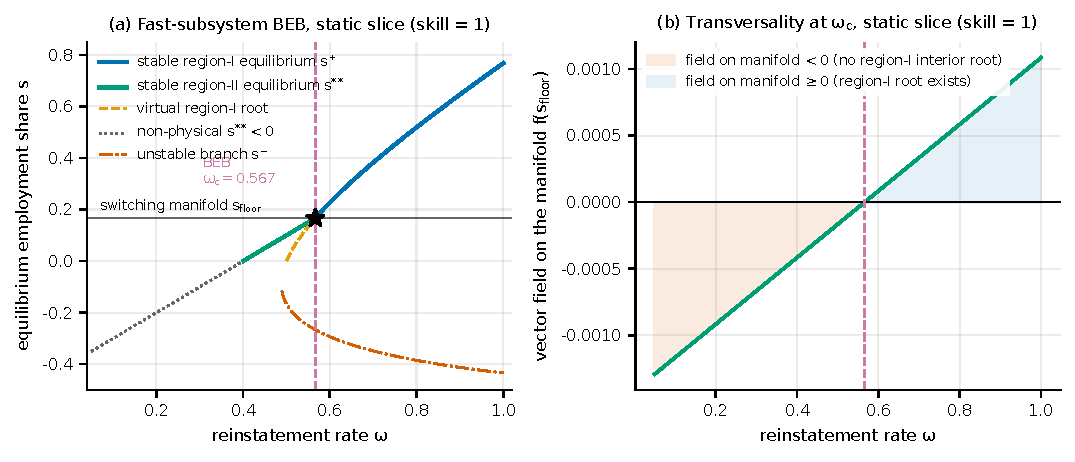
\includegraphics[width=0.98\textwidth]{fig_beb_static.pdf}
\caption{Boundary equilibrium bifurcation of the fast subsystem, static slice with skill fixed at one. Left: the physical equilibrium branch is absorbing at $s=0$ for $\omega<\kappa_I/q_A$, rises as a stable region-II (low-employment) equilibrium between $\kappa_I/q_A$ and $\omega_c$, and persists through the switching manifold $s_{\text{floor}}$ at $\omega_c=0.567$ into the stable region-I (high-employment) branch; virtual and non-physical roots are shown light. Right: the field on the manifold $f(s_{\text{floor}})$ crosses zero transversely at $\omega_c$. On a dynamic path skill depreciates, so the effective threshold is the time-varying $\omega_c(t)$ reported in Figure~\ref{fig:beb-policy}.}
\label{fig:beb-static}
\end{figure}

\subsection{Endogenous reinstatement: capability and policy as competing log-odds}
The reinstatement rate is the same endogenous variable as in the main model, equation~\eqref{eq:omega-law}, not a separate constant. Public employment, workfare and retraining reattach workers to the production of new tasks, while AGI capability erodes labor's capture. Let $EP_t$ denote public-employment headcount and $TM_t$ workfare and transfer spending; the policy reattachment stock is
\begin{equation}
\Gamma_t=\gamma_{PE}\frac{EP_{t-1}}{L^S}
+\gamma_{TM}\frac{TM_{t-1}}{wL^S}
+\gamma_R\,\text{retrain}\cdot\text{skill}_{t-1},
\label{eq:endog-gamma}
\end{equation}
and the reinstatement rate is the competitive logistic law
\begin{equation}
\boxed{\ \omega_t=\Lambda\!\left(\ell_0+\Gamma_t-\beta_A g_t\right),\quad
g_t=\ln(A_t/A_0).\ }
\label{eq:endog-omega}
\end{equation}
This specification has the required properties. The logistic keeps $\omega_t\in(0,1)$ without truncation. With no policy and no capability growth it returns the baseline $\omega_0$; capability growth, $\beta_A g_t>0$, lowers the rate, and the policy stock $\Gamma_t$ offsets that decline. Setting $\beta_A=0$ removes the capability term and recovers the policy-only limit, while the exogenous constant $\omega_t=\omega$ is the degenerate special case used for the calibrated thresholds below.

\begin{proposition}[Effective capture and the conditional crossing]
\label{prop:endog-cross}
The real bifurcation is governed by the effective capture $\omega_t\,\text{skill}_{t-1}$, not by $\omega_t$ alone. The instantaneous threshold on the nominal rate is
\[
\omega_c(t)=\frac{\kappa_I/q_A+s_{\text{floor}}}{\text{skill}_{t-1}},
\]
which rises as skill falls. A real crossing into the high-employment region requires the effective capture to reach $\kappa_I/q_A+s_{\text{floor}}$, and is therefore conditional on skill being retained. The partial effects of the two competing terms are opposite and bounded, $\partial\omega_t/\partial\Gamma_t=\omega_t(1-\omega_t)>0$ and $\partial\omega_t/\partial g_t=-\beta_A\omega_t(1-\omega_t)<0$.
\end{proposition}

\subsection{Dynamic verification and the critical policy intensity}
The conditional crossing is verified on the full system in Figure~\ref{fig:beb-policy}, with capture peaks as full-path maxima. With no policy, effective capture never exceeds $0.052$, the employment share is absorbed to zero and consumption breaks the floor ($\min C=0.057$). Under the corner, consumption is held at $0.356$ but the capture peaks at $0.121$, defending consumption without restoring the labor engine. Under the strong floor, retraining retains skill ($\sigma$ ends at $0.96$), the capture crosses at $t=35$ and employment is retained with $\min C=0.447$, a mid-horizon crossing whose durability is qualified by the $\beta_A$ sweep; at the weaker strength the capture peaks at $0.498$, still below the threshold, so the crossing is conditional on the public-employment intensity.

\begin{figure}[htbp]
\centering
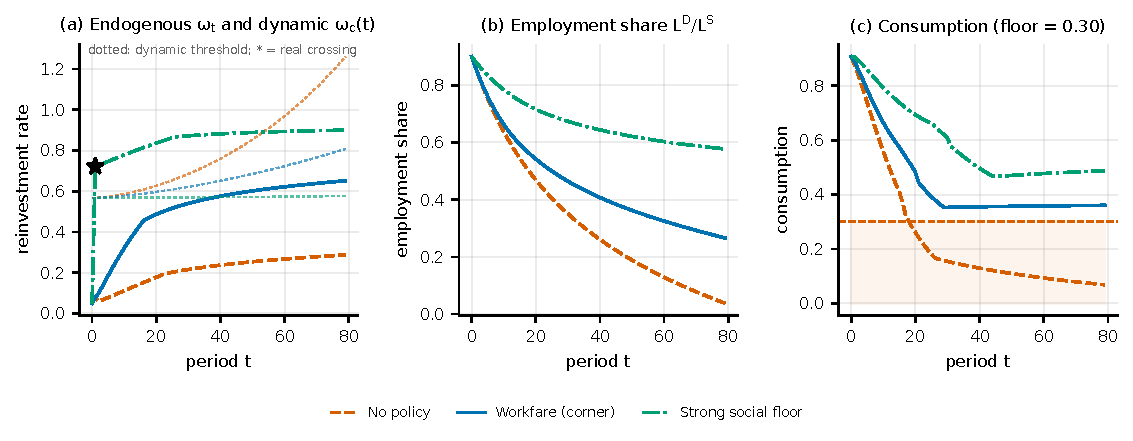
\includegraphics[width=1.0\textwidth]{fig_beb_policy.pdf}
\caption{Endogenous reinstatement and the resulting dynamic paths. (a) The endogenous rate $\omega_t$ (solid) against its instantaneous dynamic threshold $\omega_c(t)$ (dotted); the strong floor at $p_E=0.80$ crosses at $t=35$ under the baseline $\beta_A=1$ (marked $*$), while the corner and no policy stay below their thresholds. (b) Employment share and (c) consumption; the strong floor retains employment and the highest consumption, the corner holds consumption near the $0.30$ floor as market employment vanishes, and the no-policy path collapses.}
\label{fig:beb-policy}
\end{figure}

A bisection on the public-employment intensity gives the sharp threshold at which consumption is defended, defined as $\min_t C_t\ge C_{\min}$:
\begin{equation}
p_E^{*}=0.3661,
\label{eq:beb-pestar}
\end{equation}
below which the economy crashes and above which consumption is held at its floor. This is a model-implied consumption threshold, not an identified estimate or a high-employment threshold: at $p_E^*$ the effective capture does not reach the critical value, so consumption is defended by the fiscal buffer without restoring market employment. The long-horizon run confirms the distinction, with the strong-floor employment share retained at a positive but still-declining level ($s_L$ ends at $0.17$) rather than settling.

\subsection{Slow--fast dynamics and the finite-rate lag}
The endogenous rate is a slow variable and the employment share a fast
variable, $\dot s=f(s,\omega)$ and
$\dot\omega=\varepsilon\,g(\omega,\text{policy})$ with
$0<\varepsilon\ll1$, the standard singular-perturbation setup of geometric singular perturbation theory~\citep{Fenichel1979}, situated within the broader multiple-time-scale framework surveyed in the literature~\citep{Desroches2012}. Away from the switching manifold the critical manifold
is normally hyperbolic, while at the boundary equilibrium the one-sided
slopes in~\eqref{eq:bif-jump} are nonzero but unequal, so the normal
hyperbolicity is one-sided rather than lost as at a smooth fold of the kind
treated in the extended geometric theory~\citep{KS2001}; the
piecewise-smooth persistence theory for Filippov systems is the appropriate
framework. The static interior equilibrium of Theorem~\ref{thm:beb} is not
by itself an attractor of the full model. On a full path the verified
signature of an effective crossing is a discontinuous flattening of the
market-share slope, not a reversal or interior convergence: in the strong
regime the mean per-period decline of $s_L$ falls from about $-0.009$ to
about $-0.003$ while remaining strictly negative, and $s_L$ never increases.
The finite-rate lag and the full reduction are given in
Appendix~\ref{app:fast-derivation}.

\subsection{Connection to the calibrated model}
\label{subsec:connection}
The high-employment equilibrium corresponds structurally to the strong social floor, the workfare corner to the fiscally defended state as market employment vanishes, and the absorbing regime to the no-policy and pure-transfer collapses. The coefficients $\gamma_{PE},\gamma_{TM},\gamma_R$, the baseline $\omega_0$ and the capability sensitivity $\beta_A$ are structural rather than externally estimated, and the threshold $p_E^{*}=0.3661$ is a dimensionless output of the calibrated model, illustrative rather than an empirical estimate. On the corner path the region-I slope stays strictly negative, so the persistence-type classification is supported by the calibrated parameters.

The probit comparison of the share law, the $\beta_A\in\{0,1,3\}$ capability sweep and the counterfactual that removes the logistic erosion term are extended robustness runs rather than main-line results; they are reported in full in Online Appendix~D, with the probit and counterfactual reproduced by \texttt{analysis/check\_link\_function.py} and \texttt{analysis/check\_capability\_counterfactual.py}.

\subsection{Global outcome bifurcation: crash versus full public-employment absorption}
\label{subsec:global}
Under full substitution, set the public-employment policy to full absorption, the planned headcount equal to the entire unemployed population so the target share rises to one as market employment falls, while the within-period fiscal constraint is unchanged and unfunded headcount remains residual unemployment. Two outcomes follow: if the tax base expands fast enough, public employment grows in step with the released workers, residual unemployment ends at zero and the path is smooth, while if the fiscal base lags, unfunded workers accumulate and consumption breaks the floor, giving the crash basin. The boundary is the fiscal race of Proposition~\ref{prop6}, decided by whether the accumulating capital-income tax base or the collapsing wage bill leads.

A bisection on the frontier growth locates the boundary at the consumption floor. Under $\tau=0.15$ the critical value is $g_A=0.095$: grid points at $g_A=0.07$ remain smooth with $\min C=0.326$, whereas $g_A=0.10$ crashes with $\min C=0.295$. The boundary moves with the capital tax, from $g_A=0.016$ at $\tau=0.10$, through $0.095$ at $\tau=0.15$, to $0.138$ at $\tau=0.20$, after which it saturates near $g_A=0.14$ because the Laffer trade-off makes further taxation slow the growth of the very tax base it is meant to expand. Figure~\ref{fig:global-bif} maps the two basins over the $(\tau,g_A)$ plane, and Figure~\ref{fig:absorption-path} reports the smooth reallocation: market employment falls as public employment rises, residual unemployment returns to zero, and consumption stays above the floor throughout.

\begin{figure}[htbp]
\centering
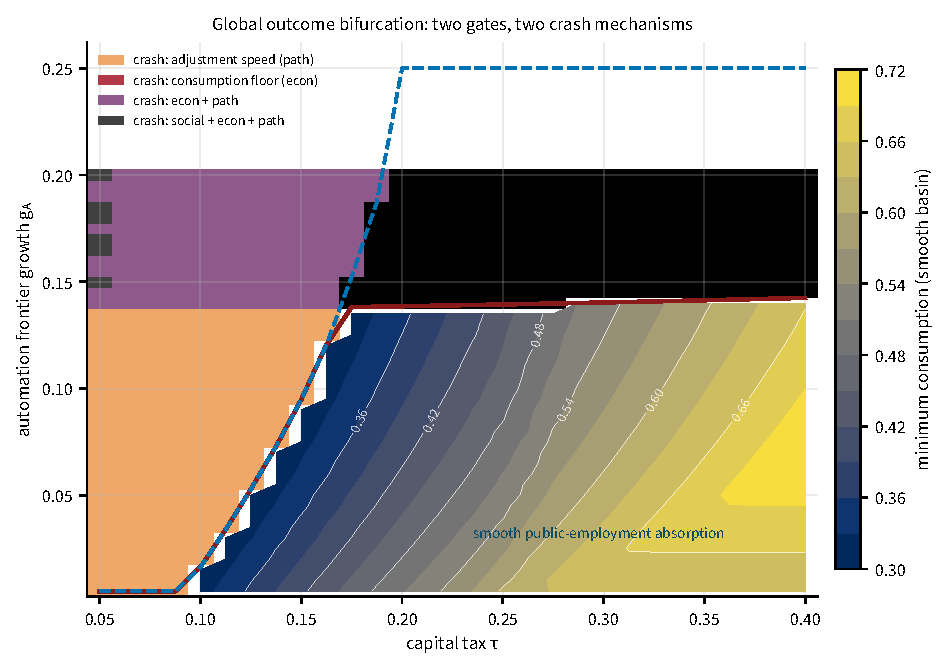
\includegraphics[width=0.95\textwidth]{fig_global_bifurcation.pdf}
\caption{Global outcome bifurcation under full absorption. The grey region is the crash basin and the colored region the smooth public-employment basin, with the color giving the minimum consumption; the dark line is the critical boundary located at the consumption floor. The boundary rises steeply with the capital tax up to $\tau\approx0.20$ and then saturates near $g_A=0.14$ through the Laffer trade-off. Keeping a transfer buffer for the unfunded residual does not move the boundary.}
\label{fig:global-bif}
\end{figure}

\begin{figure}[htbp]
\centering
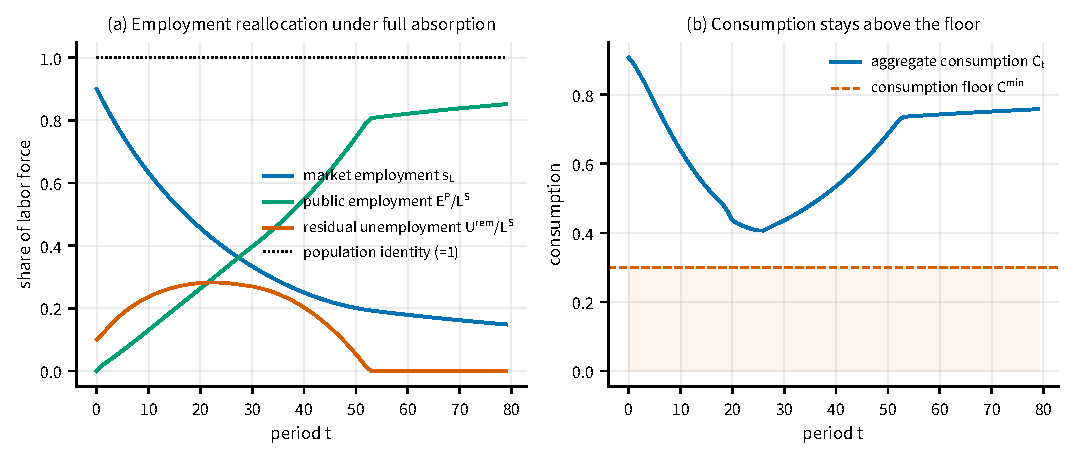
\includegraphics[width=1.0\textwidth]{fig_absorption_path.pdf}
\caption{Smooth full-absorption path at $g_A=0.010$, $\tau=0.15$. Left: market employment declines as public employment rises to absorb the released workers, residual unemployment first rises in the fiscally tight phase and then returns to zero, and the population identity stays at one. Right: consumption dips in the tight phase but remains above the floor and recovers as the tax base expands.}
\label{fig:absorption-path}
\end{figure}

The boundary is not an artifact of removing transfers. When the unfunded residual is allowed a transfer payment from the fiscal room left after public employment, the critical frontier speed under $\tau=0.15$ is unchanged at $g_A=0.095$, because in the crash basin the residual fiscal room is too small and the transfer MPC too low to hold consumption at the floor. The global bifurcation therefore rests on the fiscal race rather than on the pure-public-employment specification, and the entire set of numbers in this subsection is reproduced by \texttt{analysis/check\_full\_absorption.py}.

% ============================================================================
\section{Calibration}
\label{sec:calibration}
% ============================================================================
\subsection{Parameter--data mapping}
Standardization $L^S=\barL=1$, $w=1$. The reinstatement rate is held at its exogenous special case $\omega=0.05$ in this section, while the main model endogenizes it and reports its own threshold, the two reconciled in Section~\ref{subsec:connection}. Lowering the transfer ceiling to $\phi^{\max}=0.001$ at the corner lowers $\min_tC_t$ from $0.357$ to $0.353$, so the $0.003$ gap is the buffer carried by a two-percent transfer ceiling.

\smallskip\noindent\textbf{What ``calibration'' means here.} Three entries are anchored to data: the consumption floor ratio $c_0$ to the U.S. absolute poverty line, the transfer MPC $\mu_{TM}$ to total-consumption MPC estimates for low-liquidity recipients, not the in-kind SNAP margin, and the workfare wage ratio $w^P/w$ to workfare programmes. One group sits in a literature range on an annual-frequency convention: the model period is one year, so a quarterly Calvo no-reset probability $\zeta_q=0.75$ maps to $\zeta_y=\zeta_q^4=0.316$, a mean annual duration of $1.46$ years, and the slopes $\gamma_p,\lambda_w$ are annual-rate reduced-form conventions. The remaining entries are model-set, among which $\kappa_I$ is a calibration target set so the $T=80$ horizon reaches $s_t\to0$, not an estimated displacement rate, so the completion within 80 periods restates the target rather than tests it. The social and accounting coefficients are conventions as well. Calibrated therefore means three data-anchored magnitudes plus a two-parameter literature range, with everything else declared as setting; the parameter vector has not been estimated.

\begin{center}
\renewcommand{\arraystretch}{1.15}
\footnotesize
\begin{tabular}{@{}
>{\raggedright\arraybackslash}p{0.95in}
>{\raggedright\arraybackslash}p{1.35in}
>{\raggedright\arraybackslash}p{0.70in}
>{\raggedright\arraybackslash}p{2.80in}@{}}
\toprule
Param & Meaning & Baseline & Anchor / source \\
\midrule
$s_0=(N_0-I_0)/N_0$ & initial labor share & 0.90 & model initial state $I_0=0.20$, $N_0=2.00$ gives $s_0=0.90$; U.S.\ labor share 53.8\% is a benchmark only \emph{[model initial state; see note]} \\
$\kappa_I$ & automation displacement & 0.020 & transition (T$=$80) drives $s_t\to0$ \emph{[calibration target; set to hit $s_t\to0$ at $T{=}80$; not estimated]} \\
$g_A$ & automation frontier growth & 0.010 & long-run U.S.\ TFP $\approx1\%$/yr; the compute-cost decline is not used~\cite{HHSAI} \emph{[model-set; see note]} \\
$\eta$ & capital-tax growth inhibition & 0.40 & no direct anchor; a growth-inhibition coefficient, not a tax rate~\cite{DLL2014,OECD2026} \emph{[model-set; see note]} \\
$\gamma_p,\lambda_w$ & nominal rigidity & 0.15, 0.12 & Smets--Wouters Calvo $\zeta_p=\zeta_w=0.75$ (Nakamura--Steinsson; Bils--Klenow)~\cite{SW2007,NS2008,BK2004}; quarterly $\zeta_q=0.75\to\zeta_y=\zeta_q^4=0.316$ annual, mean duration $1.46$ years, and the two slopes are annual-rate reduced-form conventions \emph{[literature range, annual frequency]} \\
$\mu_{TM}$ & transfer MPC (total consumption) & 0.50 & total-consumption MPC out of transfers: Karger--Rajan EIP 0.46; CARES low-liquidity 0.53--0.66; Cooper--Olivei; IMF 0.20; Miller 0.44--0.55~\cite{KR2021,CO2021,HLR2025}. The USDA SNAP value 0.30 is the \emph{food-at-home} MPC (the other 0.70 is reallocated across goods, not lost to saving), so it is a different margin and is not used to anchor this total-consumption coefficient~\cite{CM2019} \emph{[literature range, total-consumption MPC]} \\
$c_0$ & consumption floor ratio & 0.30 & U.S.\ absolute poverty threshold (ASPE/HHS), divided by the baseline full-time wage income $wL^S=1$ to give the normalized floor; the historical ``food $\times3$'' origin is noted but is not the normalization used here \emph{[data-anchored level; normalization explicit]} \\
$\omega$ & reinstatement rate & 0.05 & A\&R: reinstatement weaker than displacement~\cite{AR2018} \emph{[model-set; direction grounded, magnitude not estimated]} \\
$w^P/w$ & workfare wage ratio & 0.85 & MGNREGA / World Bank workfare wages set below the market wage (direction grounded); the specific 0.85 ratio is a model setting rather than a point estimate~\cite{Subbarao2013} \emph{[direction data-grounded; level model-set]} \\
\bottomrule
\end{tabular}
\end{center}

\noindent\footnotesize\textit{Note.} The initial share $s_0=0.90$ is computed from the task block as an internal consistency requirement, with the U.S. labor income share serving only as a qualitative benchmark since $s$ is a task share and enters no equation. The frontier growth is set at the long-run TFP rate; the hardware-cost decline and efficiency gain reported by Stanford HAI and NVIDIA refer to the cost of computing rather than $A_t$ and are not used as an anchor. The coefficient $\eta$ scales the growth cost of the tax and is not an effective tax rate, so EATR levels and tax-base elasticities serve as magnitudes only. The symbol $\sigma_t$ denotes the skill stock, not a capital--labor elasticity, and the model has no CES production block; the broader elasticity ranges in task-based calibrations are background only.
\normalsize

\begin{center}
\renewcommand{\arraystretch}{1.15}
\footnotesize
\begin{tabular}{@{}
>{\raggedright\arraybackslash}p{0.95in}
>{\raggedright\arraybackslash}p{1.35in}
>{\raggedright\arraybackslash}p{0.70in}
>{\raggedright\arraybackslash}p{2.80in}@{}}
\toprule
Param & Meaning & Baseline & Anchor / source \\
\midrule
$\alpha_s$ & social-pressure coefficient & 0.60 & $\varsigma_t=\alpha_s\,U_t^{rem}/\barL$; relief share drives instability \emph{[model-set / calibration convention]} \\
$\varsigma^{th}$ & social-instability threshold & 0.50 & sustained $J=10$-period exceedance $\Rightarrow$ social collapse \emph{[model-set / calibration convention]} \\
$T$ & simulation horizon & 80 & transition window over which $s_t\to0$ is computed \emph{[model-set / calibration convention]} \\
$\delta_\sigma$ & skill depreciation & 0.015 & skill stock decay per period unemployed \emph{[model-set / calibration convention]} \\
$g_{disp}$ & automation output boost & 0.05 & $\delta_{disp}=(I_t-I_0)/N_0$ output dividend \emph{[model-set / calibration convention]} \\
$\theta$ & borrowing response to gap & 0.10 & $\theta\max\{0,C^{fe}-Y_t^d\}$ new-borrowing term in the net-flow decision \emph{[model-set / calibration convention]} \\
$\chi$ & amortization of excess debt & 0.15 & $\chi\max\{0,D_t^{roll}-\bar b P_t\}$ net deleveraging rate \emph{[model-set / calibration convention]} \\
$b^{credit}$ & bank credit ceiling & 0.80 & hard underwriting bound $D_t\le b^{credit}P_t$ on the debt burden; a stock constraint, not a consumption cut \emph{[model-set / calibration convention]} \\
$\mu_d$ & monetary drag on disposable flow & 0.06 & $-\mu_d\max\{0,r_t^d\}$ \emph{[model-set / calibration convention]} \\
$\bar b$ & debt burden target & 0.35 & target real debt in the amortization rule \emph{[model-set / calibration convention]} \\
$D_0$ & initial nominal debt (normalized) & 0.30 & initial balance sheet \emph{[model-set / calibration convention]} \\
\midrule
\multicolumn{4}{@{}p{6.3in}@{}}{\textit{Baseline policy levers (headline corner).} $\tau=0.15$, $p_E=0.45$ (workfare-dominant), $\phi^{\max}=0.02$ (the grid floor; transfers effectively closed under the baseline loss weights). This is the reported headline, which retains a buffer; the grid's mathematical minimum under the baseline weights sits at $(\tau,p_E)=(0.10,0.40)$, as explained below.} \\
\bottomrule
\end{tabular}
\end{center}

\smallskip\noindent\textbf{The transition-loss objective.}
The grid search ranks policies by a single scalar, and we therefore state that scalar explicitly instead of leaving it implicit in the simulation code. Writing $C^{fe}=w\barL$ for full-employment consumption, the objective for a policy path $(\tau,p_E,\phi^{\max})$ is
\begin{equation}
\mathcal{L}(\tau,p_E,\phi^{\max})
=\sum_{t=0}^{T}\Big[
\max(0,C^{fe}-C_t)
+\lambda\,TM_t
+\lambda_{PE}\,w^{P}EP_t+\nu\,EP_t^{2}
+\delta_\tau\,\tau^{2}\text{tax}_t
\Big],
\label{eq:loss}
\end{equation}
with $\lambda=0.5$, $\lambda_{PE}=0.6$, $\nu=0.5$ and $\delta_\tau=0.6$.
The four terms are in consumption units: the consumption gap, transfer outlays charged at the leakage rate, public-employment outlays with a congestion term, and the quadratic tax deadweight that produces the Laffer trade-off.
Feasibility is a separate criterion and is not part of $\mathcal{L}$: a path is admissible if $C_t\ge C_{\min}=c_0\,w\barL$ for every $t\ge10$, the first ten periods being excluded to remove the initial-condition transient, and the statistic $\min_tC_t$ quoted throughout the calibration (including the robustness and social-anchoring subsections) and in Figure~\ref{fig:baseline} refers to that window.
Proposition~\ref{prop3b} is the one-dimensional projection of \eqref{eq:loss}: with $p_E$ and $\phi^{\max}$ held fixed, the transfer and workfare charges collapse into its single $cost(\tau)$ term and the deadweight enters with the same quadratic form, so $W(\tau)$ and $\mathcal{L}$ rank policies identically along the $\tau$ axis.
The four weights are conventions rather than estimates, so $\mathcal{L}$ is a scenario loss index under stated weights rather than a normative welfare measure, with no household utility specified; the normative statements are confined to feasibility and financing, and the loss numbers are comparative scenario statistics.

\paragraph{External ranges for the two policy instruments} Two empirical ranges check the settings without becoming inputs. For workfare, Lee, Ko and Kim~\cite{LeeKoKim2023} estimate that one public-sector position raises private employment by one, and Gechert~\cite{Gechert2015} reports public-spending multipliers near one that exceed those of transfers; the model omits the private-employment multiplier, so adding it would raise the workfare ranking. For the pure transfer, Vivalt et al.~\cite{Vivalt2024} find a small labor-supply reduction from a guaranteed income; the model has no hours margin and holds labor supply fixed, which flatters the transfer by leaving the tax base unshrunk. Both gaps therefore run in the direction that makes the ranking harder to establish, and neither range enters an equation; this is the sense in which the policy claims are model-implied rather than universal.

\begin{figure}[htbp]
\centering
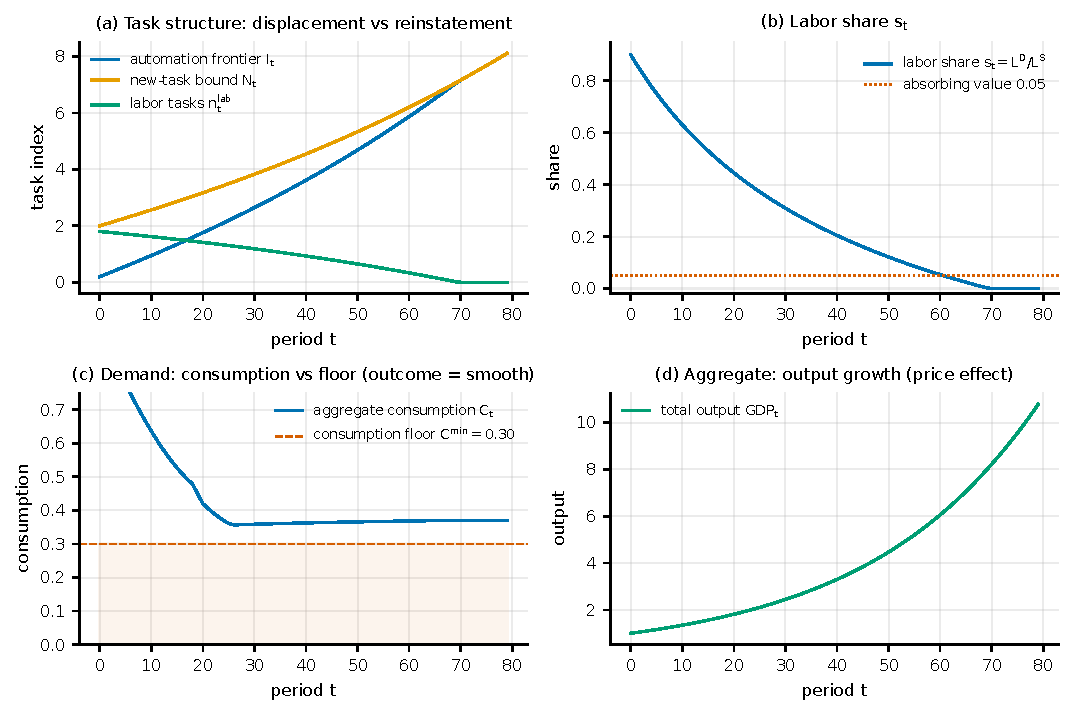
\includegraphics[width=0.98\textwidth]{fig_baseline.pdf}
\caption{Baseline smooth transition under the corner configuration $(\tau=0.15,p_E=0.45,\phi^{\max}=0.02)$ at the baseline frontier growth $g_A=0.010$. (a) The automation frontier $I_t$ and new-task bound $N_t$ diverge while labor tasks $n_t^{lab}$ vanish. (b) The labor share declines monotonically to its absorbing value. (c) Aggregate consumption stays above the floor $C^{min}=0.30$ (minimum $0.357$). (d) Total output keeps rising through the transition.}
\label{fig:baseline}
\end{figure}

\subsection{Robustness of the analytical results under the calibrated parameters}
Figure~\ref{fig:baseline} reports the baseline path under the corner configuration. Under the calibrated parameters ($\mu_{TM}=0.50$, $\eta=0.40$), transfers are costly relative to public-employment wages (one yuan of transfers yields $0.50$ of consumption, whereas a public-employment wage yields $1$), and the capital tax carries a Laffer supply-side cost. Running the full battery under the unified model engine yields the following calibrated outcomes:

\begin{center}
\small
\begin{tabular}{@{}
>{\raggedright\arraybackslash}p{1.55in}
>{\raggedright\arraybackslash}p{2.15in}
>{\raggedright\arraybackslash}p{2.45in}@{}}
\toprule
Result & Calibrated outcome & Conclusion \\
\midrule
Policy delay $d$ & corner ($\phi^{\max}{=}0.02$): $d{=}0$ and $d{=}12$ both smooth (0.357); standard ($\phi^{\max}{=}0.65$): $d{=}0$ and $d{=}12$ both smooth (0.358 and 0.366) & delay immaterial at the corner and under the standard setting \\
Isolation gain $\Delta$ vs $\omega$ & $0.018\to0.514$ & monotone, robust \\
Workfare vs pure transfer & $6/6$ not crashed ($4$ smooth/reached, $2$ not-reached) vs $6/6$ crashed & workfare $>$ transfer at every $\omega$ \\
Minimum-loss point (grid) & $(0.10,0.40,0.02)$ & corner: workfare-dominant, close transfers, low tax \\
Feasible share, $p_E{=}0.45$ vs $0.30$ & $64.1\%$ vs $26.6\%$ & advantage retained \\
No-policy / pure-transfer & crash / all crash & buffering and financing necessary \\
\bottomrule
\end{tabular}
\\[2pt]
\footnotesize The feasible share is the fraction of grid cells smooth under the operational criterion in Proposition~\ref{prop3a}: $41/64=64.1\%$ at $p_E=0.45$, $17/64=26.6\%$ at $p_E=0.30$, and $208/384=54.2\%$ overall. The workfare--transfer row is a same-fiscal comparison on identical $(\tau,\phi^{\max})$: across six $\omega$ values workfare survives all six while the pure transfer crashes all six, and of the six surviving paths four reach the target and two are not-reached, so the no-crash count is not a claim that all six reach the target.
\end{center}

\smallskip\noindent\textbf{The public-employment intensity is load-bearing.} The same six $\omega$ values survive at $p_E=0.45$ but all collapse at $p_E=0.30$, every path through the floor; the corner survives only above a share of about $0.36$, a feasibility bound rather than a tuning preference.

\begin{table}[h]
\centering\small
\caption{Structural decomposition of the pure-transfer failure. All four runs use the identical fiscal setting $(\tau=0.16,p_E=0,\phi^{\max}=0.65)$ and vary only the two structural choices the workfare corner does not share: the transfer consumption MPC $\mu_{TM}$ and the social-instability coefficient $\alpha_s$. Reproduced by \texttt{analysis/check\_transfer\_structure.py}.}\label{tab:transfer-structure}
\begin{tabular}{@{}lccc@{}}
\toprule
Configuration & outcome & crash type & $\min C$ \\
\midrule
Baseline ($\mu_{TM}=0.50,\alpha_s=0.60$) & crash & both & 0.2589 \\
Equal MPC ($\mu_{TM}=1.00$) & crash & social only & 0.4086 \\
Social disabled ($\alpha_s=0$) & crash & economic & 0.2589 \\
Both relaxed ($\mu_{TM}=1.00,\alpha_s=0$) & smooth & none & 0.4086 \\
\bottomrule
\end{tabular}
\end{table}

\noindent The decomposition separates the two mechanisms. With an equal MPC the transfer holds consumption above the floor ($\min C=0.4086$), leaving only the social channel, while with the social channel disabled but the MPC leakage retained the path still crashes economically ($\min C=0.2589$); only when both are relaxed does the regime become smooth. The workfare advantage therefore rests on the combination of the unit workfare MPC and the relief-to-jobs conversion, not on a generic financing failure, and the table states the exact conditions under which the ranking holds; the corresponding time paths of the three regimes are plotted in Figure~\ref{fig:policy-compare}.

\begin{table}[h]
\centering\small
\caption{Symmetric-limit welfare comparison on the same fiscal setting $(\tau=0.16,\phi^{\max}=0.65)$, with the transfer MPC set to one and the social channel disabled $(\mu_{TM}=1,\alpha_s=0)$. The two columns differ only in the public-employment share $p_E$. Total loss is the engine welfare loss and fiscal spend is the transfer plus workfare wage bill. Reproduced by \texttt{analysis/check\_symmetric\_welfare.py}.}\label{tab:symmetric-welfare}
\begin{tabular}{@{}lcccc@{}}
\toprule
Regime & outcome & total loss & fiscal spend & $\min C$ \\
\midrule
Public employment ($p_E=0.45$) & smooth & 55.34 & 36.12 & 0.4177 \\
Pure transfer ($p_E=0$) & smooth & 51.23 & 32.01 & 0.4086 \\
\bottomrule
\end{tabular}
\end{table}

\noindent The symmetric limit reverses both the feasibility classification and the welfare ranking, the pure transfer attaining a lower total loss ($51.23$ against $55.34$) at a lower spend ($32.01$ against $36.12$). Once the transfer MPC equals one and the social channel is disabled, a transfer yuan supports consumption as a workfare wage does, while the public-employment path still carries its workfare cost, which then dominates. This is a conditional result, the reversal requiring both $\mu_{TM}=1$ and $\alpha_s=0$ simultaneously, and the calibrated values satisfy neither; the symmetric numbers are the boundary at which the ranking changes, not the baseline case.

\smallskip\noindent\textbf{Sensitivity to $g_A$ and $\eta$.} Sweeping $g_A$ over $\{0.010,0.05,0.10,0.20,0.30\}$ gives minimum consumption $0.357,0.344,0.294,0.237,0.222$ with smooth, smooth, crash, crash, crash; the buffer holds at $g_A=0.05$, one sixth of the often quoted hardware-cost decline, and the floor is breached at $0.10$. This is the sharpest calibration sensitivity, so the smooth conclusion is conditional on a conservative long-run-TFP frontier rate rather than a hardware-cost rate. By contrast $\eta$ is nearly inert, every corner outcome smooth at $\min_tC_t=0.357$ with the total loss moving about $0.1\%$, so its imprecision affects no conclusion and no sharp Laffer effect can be claimed at $\tau=0.15$.

\begin{figure}[htbp]
\centering
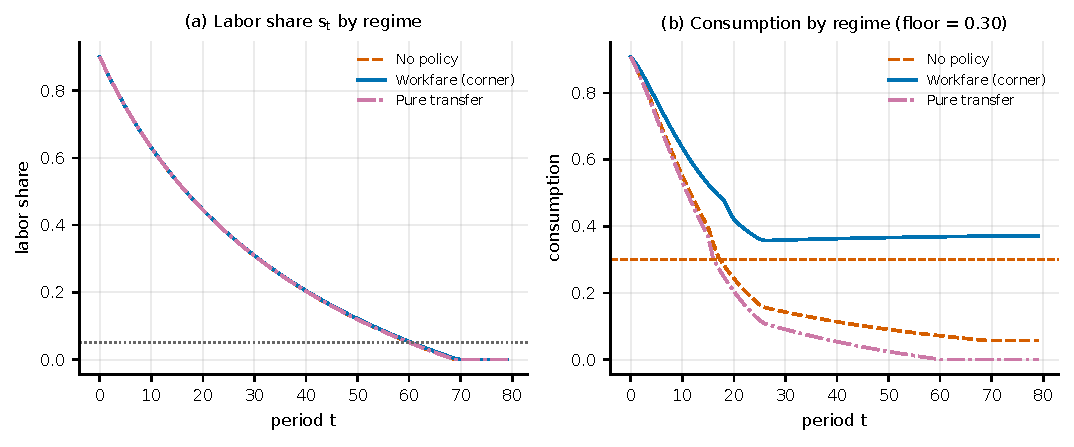
\includegraphics[width=0.98\textwidth]{fig_policy_compare.pdf}
\caption{Policy-regime comparison. Each regime carries its own fiscal setting: no policy $(\tau=0.05,\phi^{\max}=0.15)$, the workfare corner $(\tau=0.15,p_E=0.45,\phi^{\max}=0.02)$, and the pure transfer $(\tau=0,\phi^{\max}=0.65)$. This is therefore a comparison of regimes rather than a same-fiscal instrument test, which is given in the table above. (a) The labor share $s_t$ follows the same task-driven decline under all three regimes. (b) The workfare corner holds aggregate consumption above the floor, whereas the no-policy and pure-transfer regimes fall below it and become infeasible; the consumption buffer, not the market employment count, is what distinguishes the regimes.}
\label{fig:policy-compare}
\end{figure}

\smallskip\noindent\textbf{Grid minima and identification.} Figure~\ref{fig:loss-surface} visualizes the loss surface, whose minimum is at $(0.10,0.40)$ with the loss locally flat and the coordinates grid-dependent rather than sharply identified. The minimum clears the floor by only a few thousandths, so we report the better-buffered corner $(0.15,0.45,0.02)$ with $\min_t C_t=0.357$ as the headline, a deliberately conservative choice. Lowering $\phi^{\max}$ lowers the loss monotonically, so closing transfers is a preference of the objective rather than a grid artifact.

\begin{figure}[htbp]
\centering
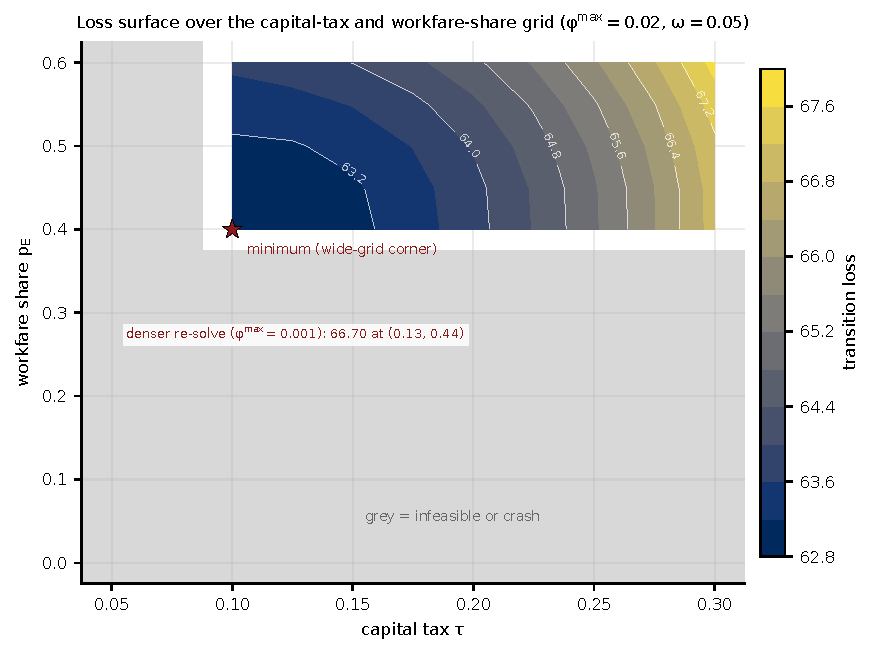
\includegraphics[width=0.92\textwidth]{fig_loss_surface.pdf}
\caption{Transition loss over the capital-tax and workfare-share grid at $\phi^{\max}=0.02$, $\omega=0.05$. The grey region is infeasible (crash); the smooth region is confined to high workfare shares, and under the baseline loss weights the loss-minimizing point on this grid sits at its corner (solid star). The smooth surface is locally flat, so the minimizer's exact coordinates are grid-dependent rather than identified. A denser re-solve that extends $\phi^{\max}$ to $0.001$ moves the minimizer to $(0.10,0.40)$ with a loss of $62.82$ (stated in the panel); that location is not a point on the $\phi^{\max}=0.02$ surface drawn here, which is why it is reported in words rather than marked.}
\label{fig:loss-surface}
\end{figure}

\smallskip\noindent\textbf{Sensitivity to the loss weights.} Feasibility is weight-independent, re-ranking all grid points under six weight configurations leaving the admissible set at $208$ points in every case, while the ranking among admissible paths depends on them. The minimizer moves across configurations, yet public employment remains the dominant instrument in every case ($p_E\in[0.30,0.55]$), whereas the transfer ceiling varies widely. Workfare dominance is therefore a property of the model, while transfers being closed at the optimum is a property of the baseline weights and the lower grid bound, reported as such.

\smallskip\noindent\textbf{Stochastic robustness.} We shock the frontier growth, the parameter on which the smooth conclusion most depends, setting $g_{A,t}=0.010+\varepsilon_t$ with an AR(1) deviation ($\rho=0.5$, Gaussian innovations of standard deviation $\sigma_\varepsilon$, distinct from the skill index $\sigma_t$); each configuration is run $200$ times and a path is recorded as a crash when it triggers a crash test before the horizon. Table~\ref{tab:shock} reports the results.

\begin{table}[h]
\centering\small
\caption{Monte Carlo crash counts under frontier-growth shocks ($200$ replications; AR(1), $\rho=0.5$). Buffer is $\min_tC_t-0.300$; the last column reports the fifth percentile of $\min_tC_t$ at $\sigma_\varepsilon=0.03$.}\label{tab:shock}
\begin{tabular}{@{}lccccc@{}}
\toprule
Configuration & buffer & $\sigma_\varepsilon{=}0.01$ & $\sigma_\varepsilon{=}0.02$ & $\sigma_\varepsilon{=}0.03$ & $\min_tC_t$, 5\% \\
\midrule
Headline $(0.15,0.45,0.02)$ & $0.056$ & $0/200$ & $0/200$ & $0/200$ & $0.3540$ \\
Refined $(0.13,0.44,0.001)$ & $0.048$ & $0/200$ & $0/200$ & $0/200$ & $0.3348$ \\
\bottomrule
\end{tabular}
\end{table}

Two things follow. First, neither configuration crashes across the tested sizes, the bounded debt block and financed buffer defending consumption; with zero crashes in $200$ draws, the Clopper--Pearson one-sided $95\%$ upper bound on the true crash probability is $1.49\%$, so zero observed crashes does not establish a zero probability. At $\sigma_\varepsilon=0.03$, $69$ headline paths ($65$ refined) fail to reach the absorbing value within $T$ and are right-censored, counted as neither survival nor crash rather than evidence of robustness. Second, the margin still separates the two: the headline buffer of $0.056$ holds the fifth-percentile minimum at $0.354$, while the refined configuration with a $0.048$ buffer falls to $0.335$, leaving consumption closer to the floor.

The deterministic v6 global-best point $(0.10,0.40,0.001)$ is not a third crash-free stochastic design. Its buffer is only $0.007$, and under the stochastic engine it crashes, with $16$, $58$ and $74$ paths at the three shock sizes and fifth-percentile minimum consumption falling to $0.298$, $0.288$ and $0.279$; consumption first breaks the floor mid-horizon after the skill stock has depreciated. The refined point $(0.13,0.44)$ keeps a $0.048$ buffer and stays crash-free, so buffer thickness rather than the third decimal of the deterministic loss decides stochastic survival. Demand-side, monetary and policy-implementation shocks are not modelled, and a fully stochastic version remains for future work.

\smallskip\noindent\textbf{Two configurations, not one.} The smooth headline depends on the public-employment intensity rather than the transfer ceiling. Under the standard setting, both workfare shares clear the floor ($\min C=0.333$ and $0.358$ at $p_E=0.30$ and $0.45$), and a higher share raises the margin; the sharp threshold for this calibration is $p_E=0.1405$. The binding condition is therefore the workfare share, not a tight transfer ceiling.

\begin{figure}[htbp]
\centering
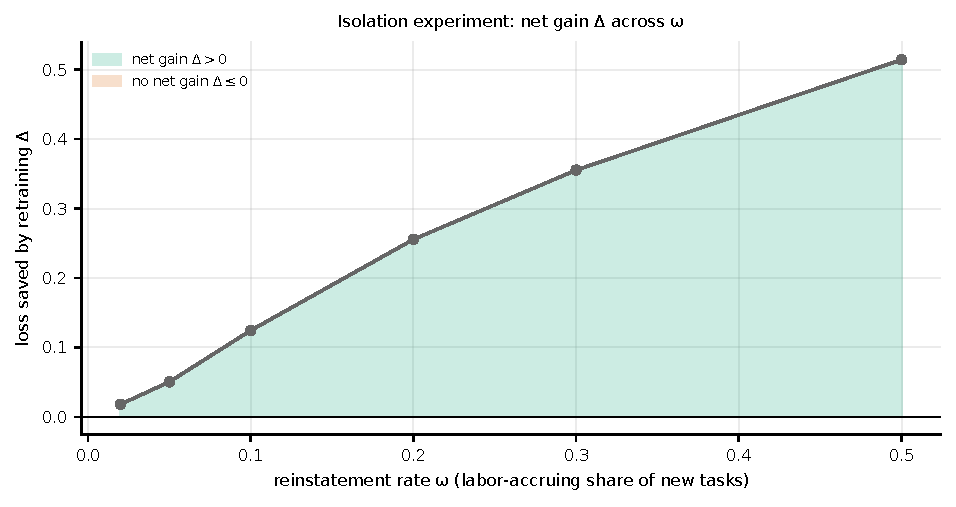
\includegraphics[width=0.84\textwidth]{fig_skill_omega.pdf}
\caption{Isolation experiment: the loss saved by retraining $\Delta$ rises monotonically with the reinstatement rate $\omega$, the share of new tasks accruing to labor. As $\omega\to0$ (AGI takes over new-task creation and reinstatement fails), the value of retraining vanishes, confirming that skill retention pays off only while labor can still capture new tasks.}
\label{fig:skill-omega}
\end{figure}

\smallskip\noindent\textbf{Social-threshold sensitivity sweep.} A dedicated sweep varies one social-channel parameter at a time ($\varsigma^{th}$, $\alpha_s$, $J$) under the calibrated parameters and compares the corner, the standard setting and the pure transfer; Table~\ref{tab:socbase} reports baseline outcomes and Table~\ref{tab:socbound} the boundaries.

\begin{table}[h]
\centering\small
\caption{Baseline social-channel outcomes ($\varsigma^{th}=0.50,\alpha_s=0.60,J=10$, $g_A=0.010$). Values within $10^{-3}$ of the floor are given to four decimals.}\label{tab:socbase}
\begin{tabular}{@{}lccccc@{}}
\toprule
Policy & outcome & crash type & $\min C$ & peak stress & social crash \\
\midrule
Corner $(0.15,0.45,0.02)$ & smooth & none & 0.357 & 0.330 & no \\
Standard $(0.16,0.45,0.65)$ & smooth & none & 0.3576 & 0.330 & no \\
Pure transfer $(0.16,0,0.65)$ & crash & both & 0.2589 & 0.600 & yes \\
\bottomrule
\end{tabular}
\end{table}

\begin{table}[h]
\centering\small
\caption{Social-crash boundaries under one-at-a-time sweeps.}\label{tab:socbound}
\begin{tabular}{@{}lccc@{}}
\toprule
Swept parameter (baseline) & Corner & Standard & Pure transfer \\
\midrule
critical $\varsigma^{th}$ (base 0.50) & $0.33$ & $0.33$ & $0.60$ \\
critical $\alpha_s$ (base 0.60) & $0.91$ & $0.91$ & $0.50$ \\
critical $J$ (base 10) & never triggers & never triggers & all $J\in[3,30]$ \\
\bottomrule
\end{tabular}
\\[2pt]
\footnotesize Values below/above the boundary trigger the social crash; for $\varsigma^{th}$ a lower value triggers, for $\alpha_s$ a higher value triggers.
\end{table}

\noindent\textbf{Mechanism.} At $p_E=0.45$, only 55\% of the unemployed remain on pure relief, so $\varsigma_t=0.55\,\alpha_s u_t$, peaking at $0.330$ at the baseline, which is 34\% below the $0.50$ cutoff; the analytic boundaries $\varsigma^{th}_{crit}=0.33$ and $\alpha_s^{crit}=0.50/0.55=0.909$ are therefore exact. Under the pure transfer, 100\% stay on relief and $\varsigma_t$ peaks at $\alpha_s=0.60>0.50$, triggering the channel at the baseline.

\noindent\textbf{Conditional conclusion.} The ranking does not flip within the scanned range. To make the corner socially crash, $\varsigma^{th}$ must fall below $0.33$ or $\alpha_s$ rise above $0.91$, while the pure transfer already crashes at the baseline, and $J$ is immaterial to the corner. The ranking remains conditional on the reduced-form cutoffs, with the external anchoring examined in Section~\ref{sec:social-anchor}.

\noindent\textbf{Robustness to the functional form and to feedback.} Two tests ask whether the ranking depends on the linear pressure law. Replacing the linear conversion with the family $g(r)=r^\gamma$ gives critical $\alpha_s$ of $0.67$, $0.91$, and $1.65$ across concave, linear and convex forms, with the linear value matching the analytic $0.909$, while the pure transfer critical value is $0.50$ under every form. Opening a pressure-to-output channel, the corner stays smooth throughout ($\min C=0.326$ at full strength), the standard setting turns economic only at full strength, and the pure transfer crashes at every strength. Under both tests the workfare corner stays smooth while the pure transfer crashes, so the ranking is not an artifact of the linear, no-feedback law; the crash boundary moving from $0.67$ to $1.65$ is reported rather than absorbed.

\subsection{External empirical anchoring of the social-instability parameters}
\label{sec:social-anchor}

The three social-instability parameters are reduced-form settings rather than
externally identified quantities. The cutoff $\varsigma^{th}$ has no direct
external anchor, while $\alpha_s$ and $J$ are only partially anchored:
crime semi-elasticities, kept in consistent units and combined with the
model's own conversion, reverse-engineer a wide illustrative interval of
about $1.0$--$6.6$ for $\alpha_s$, with the baseline $0.60$ sitting below
its lower end as a conservative setting, and $J=10$ is a mean/upper-tail
anchor drawn from crisis recovery and civil-war durations. The full
literature review, the mapping assumptions and the empirical-range sweep are
reported in Online Appendix~C. The workfare-over-transfer ranking is
conditional on these reduced-form cutoffs.

% ============================================================================
\section{Contribution to the Literature}
\label{sec:literature}
% ============================================================================
The analysis belongs to the structural-change tradition that treats technology-driven reallocation of the economy's composition, rather than a single aggregate equilibrium, as the central object. Pasinetti~\cite{Pasinetti1981} builds growth on the changing sector composition induced by technical progress, so that structural dynamics precede aggregate analysis. Goodwin~\cite{Goodwin1967} casts employment and distribution as an endogenous nonlinear cycle, studied through dynamics rather than comparative statics. Baumol~\cite{Baumol1967} shows how differential productivity growth across sectors produces structural imbalance and a persistent reallocation of labor. The present paper keeps the shared emphasis on technology-driven reallocation and nonlinear dynamics, but locates structural change at the task boundary between humans and AGI rather than at the sector boundary, and studies a case in which the reinstatement engine that reallocates displaced workers collapses endogenously rather than carrying labor through a smooth sectoral shift, with the fiscal and social safety nets closed explicitly. Against that background, the existing AGI macroeconomics literature addresses the transition along three separate axes. Restrepo (2025) and Korinek--Suh (2024) characterize the \emph{supply-side} conditions under which automation collapses wages; Fornaro--Wolf (2026) trace the \emph{demand-side} channel from income shifts to the natural rate; and the fiscal-instrument literature treats taxes and transfers as optimal-schedule objects. Within the studies surveyed here, these axes are not decided together: the size and the financing of the buffer and the existence of the high-employment branch are typically treated as separate questions. This paper proposes a two-layer task model that:

\begin{enumerate}
\item \textbf{Endogenizes the reinstatement collapse} (driven by AGI participation $\kappa_N^{AI}$ and the reinstatement rate $\omega$), proving the labor share vanishes monotonically (Theorem~\ref{thm1}), and shows skill-retention value decays with $\omega$, with no value as $\omega\to0$.
\item \textbf{Turns the Fornaro--Wolf demand shortfall into a decidable crash channel} (Theorem~\ref{thm2}), linking it to the Theorem~\ref{thm1} collapse source.
\item \textbf{Characterizes the fiscal closure}: a Laffer interior tax $\tau^*$ (Proposition~\ref{prop3b}) and within-budget superiority of public employment over transfers (Proposition~\ref{prop4}).
\item \textbf{Introduces a social-instability channel independent by construction, in a separate equation rather than through economic deflation}, proving under the assumed pressure law that workfare dominates the pure transfer for social-instability risk (Proposition~\ref{prop5}), complementing the qualitative Tcherneva/Ravallion debate and the basic-income-versus-job-guarantee comparison of Mitchell and Watts~\cite{Tcherneva,Ravallion,MitchellWatts2004}.
\item \textbf{Establishes a robustness ceiling for the buffer family} (Proposition~\ref{prop6}): strong shocks require supply-side structural measures, a result absent from the literature.
\item \textbf{States the bifurcation at two levels}. Acemoglu--Restrepo treat $\kappa_N$ (in their notation) as an exogenous constant and leave its determinants open; we derive the fast subsystem directly from the model and show that the high-employment branch reaches and crosses the switching manifold through a persistence-type boundary equilibrium bifurcation in a frozen static slice, yielding a closed-form critical reinstatement rate together with the finite-rate lag between slow policy and fast employment. Because that branch is unreachable under full substitution, we then pose the global outcome bifurcation under a full-absorption public-employment policy, locating the boundary between the crash basin and the smooth absorption basin by bisection (Section~\ref{sec:bifurcation}). Both reductions are static or model-implied statements whose parameters are dimensionless and illustrative rather than estimated; on a full path an effective fast-subsystem crossing flattens the labor-share decline discontinuously without interior convergence, so the claim is structural rather than quantitative.
\end{enumerate}

Calibration anchors three magnitudes to data (the consumption floor, the transfer MPC and the workfare wage ratio); the initial labor share $s_0=0.90$ follows from the model's own task block, the U.S.\ labor share of 53.8\% is a qualitative benchmark rather than a target, and the elasticity range and the $-$30\%/yr compute-cost decline are background and enter no equation (Section~\ref{sec:calibration}). The grid search returns a ``workfare-dominant + capital-tax-financed'' corner whose coordinates are grid-dependent rather than uniquely identified, providing an analyzable and quantitative basis for a consumption-smooth AGI transition.

Related empirical work grounds the task and labor-share foundations. The skill-content framework originates with Autor, Levy and Murnane~\cite{ALM2003}, while the automation-versus-new-tasks view of skill bias is developed by Acemoglu and Restrepo~\cite{AR2020pandp}; exposure to robots is estimated to reduce local employment and wages~\cite{AR2020}; and the globally declining labor share is documented by Karabarbounis and Neiman~\cite{KN2014} and linked to the reallocation of value toward superstar firms~\cite{ADKPV2020}. Broader policy-oriented analyses emphasize the distributional harms of AI deployed along its current trajectory~\cite{Acemoglu2021} and the need for development strategies that share the gains from artificial intelligence more widely~\cite{KS2021}.

Several recent papers address adjacent mechanisms, and in each case the difference lies along a specific axis. Atolia, Holland and Kreamer~\cite{Atolia2024} solve for the majority-voting optimal capital tax and basic income after an episode of automation, characterizing long-run outcomes and transitional welfare. Their policy is an optimal tax--transfer schedule; ours treats the two instruments as parameters of a bifurcation unfolding and asks when the high-employment branch crosses the switching manifold. Kleven and Zidar~\cite{KlevenZidar2026} characterize optimal labor and capital income taxation in a task-based automation model calibrated to the U.S. wage distribution, and find a sizable optimal capital tax that is, in their benchmark, unaffected by automation. Our capital tax is not an optimal-tax object: it is the financing instrument of the buffer. In the simulated paths capital income $\Pi_t=\max\{0,Y_t-w_tL_t^D\}$ does not shrink as $s_t\to0$; output growth outpaces the fall in the wage bill and $\Pi_t$ widens rather than contracts. The binding constraint is therefore the period-by-period timing of revenue rather than a vanishing tax base: with no reserve account, period-$t$ spending is limited to taxes already collected in $t-1$, so early in the transition, before the tax base has grown, planned spending is scaled down. The constraint we identify is this fiscal feasibility rather than tax optimality. Ray and Mookherjee~\cite{RayMookherjee2022} derive the long-run labor share in a growth framework where automation moves the share along a smooth path; we study the case in which the reinstatement engine itself collapses, so the share crosses the switching manifold through a boundary bifurcation rather than following a continuous decline. Nakamura and Zeira~\cite{NakamuraZeira2024} analyze transitional unemployment dynamics and identify conditions under which assistance arrives in time; their object is the unemployment stock, ours is the existence of an equilibrium branch. Bond and Kremens~\cite{BondKremens2024} characterize income and inequality under asymptotically full automation, a steady-state distribution question, whereas our constraint is fiscal feasibility along the transition. Jacobs~\cite{Jacobs2023} studies capitalist--worker wealth distribution in a task-based model without a policy-instrument bifurcation, and Stiefenhofer~\cite{Stiefenhofer2025} analyzes AGI substitution inside a CES production structure, where substitution is continuous across factors; our production structure is task-based, so substitution occurs at task boundaries and the resulting instability is discrete. Brault, Haghighi and Yang~\cite{BHY2026} study monetary policy in a two-sector New Keynesian model with downward nominal wage rigidity and show that accommodating AI-driven unemployment opens an intersectoral inflation wedge because one policy rate cannot clear both labor markets; their analysis is a single-instrument monetary trade-off, whereas our buffer is a fiscal instrument whose financing and the existence of the high-employment branch are decided together.

% ============================================================================
\section{Conclusion}
\label{sec:conclusion}
% ============================================================================
This paper has integrated the supply, demand, fiscal and social sides of the AGI labor transition in one numerically solvable system. The mechanism group delivers the two failure modes, a monotonic labor-share collapse that under full substitution drives market employment to zero and makes a high-employment endpoint unreachable (the counterfactual evidence is compiled in Appendix~\ref{app:high-employment}), together with a decidable demand-side spiral. The fiscal group establishes that a financed buffer is nonempty, ranks workfare above transfers within the budget and under the assumed pressure law, and bounds the buffer at a ceiling beyond which only supply-side measures help. On the method, the fast-subsystem boundary equilibrium bifurcation gives a closed-form critical rate, and the global outcome bifurcation separates the crash and smooth full-absorption basins by a fiscal race, with a critical frontier speed near $g_A=0.095$ under $\tau=0.15$ that saturates near $0.14$.

The policy implications follow within this calibrated model rather than as universal claims. At the baseline frontier growth, the smooth full-absorption path keeps minimum consumption at $0.407$ as public employment rises to $0.85$ and residual unemployment reaches zero, while the fixed corner holds consumption at $0.357$ and the no-policy path crashes at $0.057$. The loss-minimizing design is workfare-dominant and financed by a minimal sufficient capital tax, with transfers closed because their MPC leakage makes them costlier. The pure transfer and no-policy regimes are infeasible, the structural conditions being stated in Table~\ref{tab:transfer-structure}, and the absorption is conditional on the automation pace and fiscal base, the floor breached once the frontier speed crosses the critical value near $0.095$. For sufficiently fast automation no demand-side absorption can keep pace within the model, so the response indicated by the model lies on the supply side.

Seven limitations point to future work. First, the social-instability channel is reduced-form and would benefit from a microfoundation in dignity and acceptability. Second, the reinstatement rate and the frontier growth require sharper empirical calibration. Third, the model is closed-economy and abstracts from monetary policy beyond the zero lower bound; monetary-fiscal interaction and open-economy flows are natural extensions. Fourth, the core model is deterministic. The shock experiment finds neither configuration crashes at the tested scales while about a third of paths are right-censored rather than robust, and demand-side and policy-implementation shocks remain absent; a full stochastic version is left to future work. Fifth, the social-instability parameters lack strict external identification, the anchoring status and the empirical-range sweep being reported in Section~\ref{sec:social-anchor}, and the underlying empirical samples differ institutionally from the modeled setting. Sixth, both bifurcation results are model-implied rather than externally identified, the high-employment branch a counterfactual and the global boundary and $p_E^*$ dimensionless outputs of the calibrated model. Seventh, the model is partial-equilibrium: after-tax capital income and the unconsumed transfer share are recorded as non-returning leakages, with no capital-owner recycling and an exogenous credit line; endogenizing capital-owner demand and the funding side of credit could only strengthen aggregate demand.

% ============================================================================
\section*{Funding}
% ============================================================================

This research did not receive any specific grant from funding agencies in the public, commercial, or not-for-profit sectors.

% ============================================================================
\section*{Declaration of competing interest}
% ============================================================================

The author declares that there are no known competing financial interests or personal relationships that could have appeared to influence the work reported in this paper.

% ============================================================================
\section*{Declaration of generative AI and AI-assisted technologies in the writing process}
% ============================================================================

During the preparation of this work the author used a generative AI assistant in order to improve the language and readability of the manuscript. After using this tool, the author reviewed and edited the content as needed and takes full responsibility for the content of the publication.

% ============================================================================
\section*{Data availability}
% ============================================================================

The simulation code, parameter files and scripts that generate every reported number are publicly available at \url{https://github.com/whxhkwj/AGI-transition-workfare-UBI}.
% ============================================================================
\begin{thebibliography}{99}
\enlargethispage{5\baselineskip}

\bibitem{Acemoglu2021} D. Acemoglu, \emph{Harms of AI}, NBER Working Paper 29247, 2021 (Oxford Handbook of AI Governance), available at \url{https://www.nber.org/papers/w29247}.

\bibitem{AR2018} D. Acemoglu and P. Restrepo, The Race between Man and Machine: Implications of Technology for Growth, Factor Shares, and Employment, \emph{American Economic Review} 108(6), 1488--1542, 2018, DOI: \texttt{10.1257/aer.20160696}.

\bibitem{AR2020} D. Acemoglu and P. Restrepo, Robots and Jobs: Evidence from US Labor Markets, \emph{Journal of Political Economy} 128(6), 2188--2244, 2020, DOI: \texttt{10.1086/705716}.

\bibitem{AR2020pandp} D. Acemoglu and P. Restrepo, Unpacking Skill Bias: Automation and New Tasks, \emph{AEA Papers and Proceedings} 110, 356--361, 2020, DOI: \texttt{10.1257/pandp.20201063}.

\bibitem{Atolia2024} M. Atolia, M. Holland and J. Kreamer, Optimal Taxes and Basic Income during an Episode of Automation: A Worker's Perspective, \emph{Macroeconomic Dynamics} 29, e28, 1--27, 2024, DOI: \texttt{10.1017/S1365100524000361}.

\bibitem{ADKPV2020} D. Autor, D. Dorn, L. F. Katz, C. Patterson and J. Van Reenen, The Fall of the Labor Share and the Rise of Superstar Firms, \emph{Quarterly Journal of Economics} 135(2), 645--709, 2020, DOI: \texttt{10.1093/qje/qjaa004}.

\bibitem{ALM2003} D. H. Autor, F. Levy and R. J. Murnane, The Skill Content of Recent Technological Change: An Empirical Exploration, \emph{Quarterly Journal of Economics} 118(4), 1279--1333, 2003, DOI: \texttt{10.1162/003355303322552801}.

\bibitem{BK2004} M. Bils and P. J. Klenow, Some Evidence on the Importance of Sticky Prices, \emph{Journal of Political Economy} 112(5), 947--985, 2004, DOI: \texttt{10.1086/422559}.

\bibitem{BondKremens2024} P. Bond and L. Kremens, Income and Inequality under Asymptotically Full Automation, Working paper, University of Washington, 2024 (revised 2026), available at \url{https://faculty.washington.edu/apbond/research/260324%20Automation.pdf}.

\bibitem{CM2019} P. Canning and R. Mentzer Morrison, Quantifying the Impact of SNAP Benefits on the U.S. Economy and Jobs, \emph{USDA ERS Amber Waves}, July 2019, available at \url{https://www.ers.usda.gov/amber-waves/2019/july/quantifying-the-impact-of-snap-benefits-on-the-u-s-economy-and-jobs/}.

\bibitem{KR2021} E. Karger and A. Rajan, Heterogeneity in the Marginal Propensity to Consume: Evidence from Covid-19 Stimulus Payments, Federal Reserve Bank of Chicago Working Paper No. 2020-15, revised 2021, available at \url{https://www.chicagofed.org/publications/working-papers/2020/2020-15}.

\bibitem{CO2021} D. H. Cooper and G. P. Olivei, \emph{High-Frequency Spending Responses to Government Transfer Payments}, Federal Reserve Bank of Boston Research Department Working Paper 21-10, 2021, DOI: \texttt{10.29412/res.wp.2021.10}.

\bibitem{diBernardo2008} M. di Bernardo, C. J. Budd, A. R. Champneys and P. Kowalczyk, \emph{Piecewise-smooth Dynamical Systems: Theory and Applications}, Applied Mathematical Sciences vol.~163, Springer-Verlag, London, 2008, DOI: \texttt{10.1007/978-1-84628-708-4}.

\bibitem{DLL2014} M. Devereux, L. Liu and S. Loretz, The Elasticity of Corporate Taxable Income: New Evidence from UK Tax Records, \emph{American Economic Journal: Economic Policy} 6(2), 19--53, 2014, DOI: \texttt{10.1257/pol.6.2.19}.

\bibitem{FW2026} L. Fornaro and M. Wolf, Macroeconomic Policies for AI, Economics Working Paper No.~1943, Universitat Pompeu Fabra, April 2026, available at \url{https://econ-papers.upf.edu/papers/1943.pdf}.

\bibitem{BHY2026} J. Brault, M. Haghighi and J. Yang, Monetary Policy in an AI-Driven Two-Speed Economy, Bank of Canada Staff Working Paper 2026-27, July 2026, DOI: \texttt{10.34989/swp-2026-27}, available at \url{https://www.bankofcanada.ca/2026/07/staff-working-paper-2026-27/}.

\bibitem{Jacobs2023} A. Jacobs, Capitalist--Worker Wealth Distribution in a Task-Based Model of Automation, Working Paper 23/1064, Department of Economics, Ghent University, 2023, available at \url{http://wps-feb.ugent.be/Papers/wp_23_1064.pdf}.

\bibitem{HLR2025} M. Hadzi-Vaskov, E. Luttini and L. A. Ricci, \emph{Micro-Evidence on the Consumption Impact of Income-Support Policies During COVID-19}, IMF Working Paper 2025/064, 2025, available at \url{https://www.imf.org/en/publications/wp/issues/2025/04/04/micro-evidence-on-the-consumption-impact-of-income-support-policies-during-covid-19-565741}.

\bibitem{KN2014} L. Karabarbounis and B. Neiman, The Global Decline of the Labor Share, \emph{Quarterly Journal of Economics} 129(1), 61--103, 2014, DOI: \texttt{10.1093/qje/qjt032}.

\bibitem{KlevenZidar2026} H. Kleven and O. M. Zidar, \emph{Automation and Optimal Taxation: A Task-Based Theory}, NBER Working Paper 35747, September 2026, DOI: \texttt{10.3386/w35747}, available at \url{https://www.nber.org/papers/w35747}.

\bibitem{KS2021} A. Korinek and J. E. Stiglitz, \emph{Artificial Intelligence, Globalization, and Strategies for Economic Development}, NBER Working Paper 28453, 2021, available at \url{https://www.nber.org/papers/w28453}.

\bibitem{KS2024} A. Korinek and D. Suh, \emph{Scenarios for the Transition to AGI}, NBER Working Paper 32255 / arXiv:2403.12107, 2024, available at \url{https://www.nber.org/papers/w32255}.

\bibitem{MitchellWatts2004} W. Mitchell and M. Watts, A Comparison of the Macroeconomic Consequences of Basic Income and Job Guarantee Schemes, CofFEE Working Paper 04-05, Centre of Full Employment and Equity, University of Newcastle, July 2004, available at \url{http://www.basicincome.org/bien/pdf/2004WattsMitchell.pdf}.

\bibitem{NakamuraZeira2024} H. Nakamura and J. Zeira, Automation and Unemployment: Help Is on the Way, \emph{Journal of Economic Growth} 29, 215--250, 2024, DOI: \texttt{10.1007/s10887-023-09233-9}.

\bibitem{NS2008} E. Nakamura and J. Steinsson, Five Facts about Prices: A Reevaluation of Menu Cost Models, \emph{Quarterly Journal of Economics} 123(4), 1415--1464, 2008, DOI: \texttt{10.1162/qjec.2008.123.4.1415}.

\bibitem{OECD2026} OECD, \emph{Corporate Tax Statistics 2026}, OECD Publishing, Paris, 2026, available at \url{https://www.oecd.org/en/publications/corporate-tax-statistics-2026\_73af6222-en.html}.

\bibitem{Ravallion} A. Alik-Lagrange and M. Ravallion, Workfare versus Transfers in Rural India, \emph{World Development} 112, 244--258, 2018, DOI: \texttt{10.1016/j.worlddev.2018.08.008}.

\bibitem{RayMookherjee2022} D. Ray and D. Mookherjee, Growth, Automation and the Long-Run Share of Labor, \emph{Review of Economic Dynamics} 46, 1--26, 2022, DOI: \texttt{10.1016/j.red.2021.09.003}.

\bibitem{Restrepo2025} P. Restrepo, \emph{We Won't be Missed: Work and Growth in the AGI World}, NBER Working Paper 34423, 2025 (also in \emph{The Economics of Transformative AI}, University of Chicago Press), available at \url{https://www.nber.org/papers/w34423}.

\bibitem{SW2007} F. Smets and R. Wouters, Shocks and Frictions in US Business Cycles: A Bayesian DSGE Approach, \emph{American Economic Review} 97(3), 586--606, 2007, DOI: \texttt{10.1257/aer.97.3.586}.

\bibitem{Stiefenhofer2025} P. Stiefenhofer, The Future of Work and Capital: Analyzing AGI in a CES Production Model, arXiv:2502.07044, 2025, available at \url{https://arxiv.org/abs/2502.07044}.

\bibitem{Subbarao2013} K. Subbarao, C. Del Ninno, C. Andrews and C. Rodr\'iguez-Alas, \emph{Public Works as a Safety Net: Design, Evidence, and Implementation}, World Bank Directions in Development, 2013, available at \url{https://documents.worldbank.org/en/publication/documents-reports/documentdetail/289871468339050938}.

\bibitem{Tcherneva} P. Tcherneva, \emph{The Case for a Job Guarantee}, Polity Press, 2020.

\bibitem{HHSAI} Stanford HAI, \emph{Artificial Intelligence Index Report 2025}, Stanford University, 2025, available at \url{https://hai.stanford.edu/ai-index/2025-ai-index-report}.

\bibitem{GH1983} J. Guckenheimer and P. Holmes, \emph{Nonlinear Oscillations, Dynamical Systems, and Bifurcations of Vector Fields}, Springer-Verlag, New York, 1983.

\bibitem{Kuznetsov2023} Y. A. Kuznetsov, \emph{Elements of Applied Bifurcation Theory}, 4th edition, Applied Mathematical Sciences vol.~112, Springer, Cham, 2023, DOI: \texttt{10.1007/978-3-031-22007-4}.

\bibitem{Sotomayor1973} J. Sotomayor, Generic Bifurcations of Dynamical Systems, in M.~M. Peixoto (ed.), \emph{Dynamical Systems} (Proceedings of a Symposium held at the University of Bahia, 1971), Academic Press, New York, 1973, pp.~561--582.

\bibitem{Fenichel1979} N. Fenichel, Geometric Singular Perturbation Theory for Ordinary Differential Equations, \emph{Journal of Differential Equations} 31(1), 53--98, 1979, DOI: \texttt{10.1016/0022-0396(79)90152-9}.

\bibitem{KS2001} M. Krupa and P. Szmolyan, Extending Geometric Singular Perturbation Theory to Nonhyperbolic Points---Fold and Canard Points in Two Dimensions, \emph{SIAM Journal on Mathematical Analysis} 33(2), 286--314, 2001, DOI: \texttt{10.1137/S0036141099360919}.

\bibitem{Desroches2012} M. Desroches, J. Guckenheimer, B. Krauskopf, C. Kuehn, H. M. Osinga and M. Wechselberger, Mixed-Mode Oscillations with Multiple Time Scales, \emph{SIAM Review} 54(2), 211--288, 2012, DOI: \texttt{10.1137/100791233}.

\bibitem{Gechert2015} S. Gechert, What Fiscal Policy Is Most Effective? A Meta-Regression Analysis, \emph{Oxford Economic Papers} 67(3), 553--580, 2015, DOI: \texttt{10.1093/oep/gpv027}.

\bibitem{LeeKoKim2023} H. Lee, C. Ko and W. Kim, Local Employment Multiplier: Evidence from Relocation of Public-Sector Entities in South Korea, CESifo Working Paper 10870, 2023.

\bibitem{Vivalt2024} E. Vivalt, E. Rhodes, A. W. Bartik, D. E. Broockman, P. Krause and S. Miller, The Employment Effects of a Guaranteed Income: Experimental Evidence from Two U.S. States, NBER Working Paper 32719, 2024, available at \url{https://www.nber.org/papers/w32719}.

\bibitem{Pasinetti1981} L. L. Pasinetti, \emph{Structural Change and Economic Growth: A Theoretical Essay on the Dynamics of the Wealth of Nations}, Cambridge University Press, Cambridge, 1981.

\bibitem{Goodwin1967} R. M. Goodwin, A Growth Cycle, in C. H. Feinstein (ed.), \emph{Socialism, Capitalism and Economic Growth: Essays Presented to Maurice Dobb}, Cambridge University Press, Cambridge, 1967, pp.~54--58.

\bibitem{Baumol1967} W. J. Baumol, Macroeconomics of Unbalanced Growth: The Anatomy of Urban Crisis, \emph{American Economic Review} 57(3), 415--426, 1967.

\end{thebibliography}

% ============================================================================
\appendix
\section{The high market-employment counterfactual}
\label{app:high-employment}
% ============================================================================
The body treats a high market-employment endpoint as a counterfactual under
incomplete substitution. This appendix reports the falsification runs behind
that classification rather than asserting it. The normative statement that AGI
displaces every task under full substitution is Theorem~\ref{thm1}; the
question here is operational: across the full-substitution parameter domain,
does any policy configuration hold the market share at a high level at the
terminal date? A high market-employment endpoint is defined as a terminal
market share at or above $0.50$. The full battery is reproduced by
\texttt{analysis/check\_high\_employment\_unreachable.py}, which exits with all
checks passing.

\begin{center}
\small
\begin{tabular}{@{}lccc@{}}
\toprule
Configuration (full substitution) & outcome & terminal $s_L$ & terminal $E^P$ \\
\midrule
No policy ($\tau=0.05,p_E=0$)            & crash       & 0.000 & 0.000 \\
Workfare corner ($p_E=0.45$)             & smooth      & 0.004 & 0.448 \\
Strong floor ($p_E=0.80$, retrain $0.8$) & not reached & 0.338 & 0.529 \\
All levers maxed ($p_E=0.95$, retrain $1$) & not reached & 0.427 & 0.545 \\
Full absorption                          & smooth      & 0.148 & 0.852 \\
\midrule
\multicolumn{4}{@{}l@{}}{Exogenous reinstatement rate (incomplete-substitution counterfactual)} \\
$\omega=0.30$                            & not reached & 0.110 &  \\
$\omega=0.50$                            & not reached & 0.246 &  \\
$\omega=0.70$                            & not reached & 0.390 &  \\
$\omega=0.90$                            & not reached & 0.543 &  \\
\bottomrule
\end{tabular}
\end{center}

Three facts follow. First, no configuration in the full-substitution domain
reaches the $0.50$ threshold; even with every policy lever raised at once the
terminal share stays below $0.43$. Second, the paths that stay smooth do so
with a low terminal market share, the corner and full-absorption cases below
$0.15$, supported by public employment rather than by market jobs. Third, the
high-employment share is recovered only by an exogenous high reinstatement
rate, and the terminal share rises monotonically with that rate, crossing
$0.50$ near $\omega=0.90$. A high market-employment attractor is therefore a
property of the incomplete-substitution counterfactual rather than a reachable
basin of the full-substitution model.

% ============================================================================
\section{Fast-subsystem technical derivation}
\label{app:fast-derivation}
% ============================================================================
This appendix collects the algebra summarized in
Section~\ref{sec:bifurcation}: the quadratic fast field, the switching
manifold, the proof of the boundary equilibrium bifurcation, and the
slow--fast reduction. The statements are the same as in the body; only the
intermediate steps are moved here.

\paragraph{B.1 Normalization and the quadratic vector field.}
Freeze the slowly evolving state and normalize
\begin{equation}
k_h=\frac{\kappa_N^h}{N},\qquad q_A=\kappa_N^{AI}M_0,\qquad
\mu=\frac{A}{N},\qquad s=\frac{n}{N},\qquad \sigma=\text{skill},
\label{app:norm}
\end{equation}
so the task and labor-task growth are
\begin{equation}
\frac{\dot N}{N}=k_hS_0\bigl(1-\lambda_h(1-s)\bigr)+q_A\mu,\qquad
\frac{\dot n}{N}=\omega\sigma\,\frac{\dot N}{N}-\kappa_I\mu.
\label{app:growth}
\end{equation}
Using the direct automation flow that binds in the high-employment region and
$\dot s=\dot n/N-s\,\dot N/N$, expansion gives the fast field
\begin{equation}
\dot s=f_1(s)=-Cs^2+Bs+A,
\label{app:fast}
\end{equation}
with coefficients
\begin{align}
C&=k_hS_0\lambda_h>0, & \Xi&=k_hS_0(1-\lambda_h)<0,\nonumber\\
B&=C\omega\sigma-\Xi-q_A\mu, &
A&=\omega\sigma(\Xi+q_A\mu)-\kappa_I\mu.
\label{app:coeff}
\end{align}
The leading nonlinearity is quadratic and $f_1'''(s)\equiv0$, so no cubic
coefficient on which a cusp normal form would rest is induced. The generic
unfolding of a one-dimensional quadratic field is fold-type, but the event is
located here by the boundary of the admissible state space rather than by an
interior discriminant.

\paragraph{B.2 The switching manifold.}
The truncated human share $S^h(s)=S_0\max\{0,1-\lambda_h(1-s)\}$ is positive
only above $s_{\text{floor}}=1-1/\lambda_h$. Below it the human share is
identically zero and the second-region field is linear,
\begin{equation}
\dot s=f_2(s)=\mu\bigl(\omega\sigma q_A-\kappa_I-q_A s\bigr).
\label{app:f2}
\end{equation}
The fields join continuously on the manifold, and direct subtraction gives the
constant jump
\begin{equation}
f_1'(s_{\text{floor}})-f_2'(s_{\text{floor}})
=k_hS_0\bigl(\lambda_h\omega\sigma-\lambda_h+1\bigr),
\label{app:jump}
\end{equation}
so the fast subsystem is a continuous piecewise-smooth Filippov system, $C^0$
but not $C^1$.

\paragraph{B.3 Proof of the boundary equilibrium bifurcation.}
On the manifold,
\begin{equation}
f_1(s_{\text{floor}})=f_2(s_{\text{floor}})
=\mu\bigl(\omega\sigma q_A-\kappa_I-q_A s_{\text{floor}}\bigr).
\label{app:proof1}
\end{equation}
For $\mu>0$ the condition $f_1(s_{\text{floor}})=0$ is equivalent to
$\omega\sigma=\kappa_I/q_A+s_{\text{floor}}$, giving
$\omega_c=\sigma^{-1}(\kappa_I/q_A+s_{\text{floor}})$. Differentiating
\eqref{app:proof1} in $\omega$ gives $\partial_\omega f_1(s_{\text{floor}})
=\mu q_A\sigma>0$, which establishes transversality. The unique region-II
equilibrium of $f_2$ is
\begin{equation}
s^{**}=\omega\sigma-\frac{\kappa_I}{q_A},
\label{app:s2star}
\end{equation}
which equals $s_{\text{floor}}$ at $\omega_c$ and lies below the manifold for
$\omega<\omega_c$. At the boundary equilibrium the region-II slope is
$f_2'(s_{\text{floor}})=-q_A\mu<0$, and using \eqref{app:jump} at the
critical value the region-I slope is
\begin{equation}
f_1'(s_{\text{floor}})=-q_A\mu+\frac{C\kappa_I}{q_A}.
\label{app:slope}
\end{equation}
It is negative exactly under $q_A\mu>C\kappa_I/q_A$. When this persistence
condition holds, both one-sided slopes are negative and the equilibrium crosses
with stability preserved, the persistence-type BEB; if it fails, the region-I
branch is repelling and the event is not of persistence type. The hard lower
boundary contributes the entry threshold
$\omega_0^{(\text{entry})}=\sigma^{-1}\kappa_I/q_A$ at which $s^{**}=0$;
below it the physical state space contains no equilibrium and the trajectory
is absorbed at $s=0$.

\paragraph{B.4 Slow--fast reduction and the finite-rate lag.}
With $\omega$ slow and $s$ fast,
\begin{equation}
\dot s=f(s,\omega),\qquad \dot\omega=\varepsilon\,g(\omega,\text{policy}),
\qquad 0<\varepsilon\ll1,
\label{app:slow}
\end{equation}
the critical manifold $f=0$ is normally hyperbolic away from the switching
manifold because the fast slope is nonzero. At the boundary equilibrium the
one-sided slopes are both nonzero but unequal, so normal hyperbolicity is
one-sided rather than lost as at a smooth fold, and piecewise-smooth
persistence theory applies rather than the fold-type framework. The lag in the
simulations has two sources: the slow variable moves at the finite rate
$\varepsilon$, so the fast variable tracks a moving equilibrium with a
relaxation lag, and crossing the manifold changes the tracking slope
discontinuously. The static interior equilibrium is not by itself an attractor
of the full model; on a full path the verified signature of an effective
crossing is a discontinuous flattening of the market-share slope, not a
reversal or interior convergence.

\end{document}
